\documentclass[11pt,a4paper]{report}
\usepackage[a4paper,top=2.5cm,bottom=2.5cm,left=2.5cm,right=2.5cm]{geometry}
\usepackage{graphicx}
\usepackage{float}
\usepackage{tikz}
\usetikzlibrary{calc}
\usepackage{setspace}
\usepackage[nottoc]{tocbibind}
\usepackage{booktabs}
\usepackage{multirow}
\usepackage{amsmath}
\usepackage{amssymb}
\usepackage{caption}
\usepackage{subcaption}
\usepackage[hidelinks]{hyperref}
\usepackage{fontspec}
\usepackage{polyglossia}
\setdefaultlanguage{vietnamese}
\setmainfont{Times New Roman}

\setstretch{1.15}
\setlength{\parskip}{6pt}
\setlength{\parindent}{0pt}
\newcommand{\figwidth}{0.85\textwidth}

\begin{document}

% ======================= TRANG BÌA ==========================
\begin{titlepage}
\thispagestyle{empty}
\centering
\begin{tikzpicture}[remember picture, overlay]
  \draw[line width=0.8pt]
    ($(current page.north west) + (2cm,-2cm)$)
    rectangle
    ($(current page.south east) + (-2cm,2cm)$);
\end{tikzpicture}

{\bfseries\large ĐẠI HỌC KHOA HỌC VÀ CÔNG NGHỆ HÀ NỘI\par}
\vspace{4pt}
{\bfseries\large KHOA CÔNG NGHỆ THÔNG TIN VÀ TRUYỀN THÔNG\par}

\vspace{2.4cm}
\IfFileExists{figures/logo.png}{
  
\includegraphics[width=6cm]{figures/logo.png}\par
}{
  \vspace*{3.5cm}
}
\vspace{1.8cm}

{\bfseries\Large BÁO CÁO KHÓA LUẬN TỐT NGHIỆP\par}
\vspace{10pt}
{\bfseries\Large Nhận dạng Tự động các Pha Phẫu thuật trong Video Cắt Túi mật: So sánh Ba Kiến trúc Học sâu Hiện đại trên Tập dữ liệu Cholec80\par}

\vspace{2.0cm}
\begin{tabular}{@{}rl@{}}
\textbf{Sinh viên thực hiện:} & Nguyễn Trọng Bách\\[10pt]
\textbf{Giảng viên hướng dẫn:} & TS. Vũ Trọng Sinh\\
\end{tabular}

\vfill
{\large Tháng 6 năm 2026\par}
\end{titlepage}

% ======================= LỜI CẢM ƠN ==========================
\chapter*{Lời cảm ơn}
\addcontentsline{toc}{chapter}{Lời cảm ơn}

Trước hết, tôi xin bày tỏ lòng biết ơn chân thành đến giảng viên hướng dẫn của tôi, TS.~Vũ Trọng Sinh, vì những chỉ dẫn quý báu, sự hỗ trợ liên tục và kiến thức sâu rộng của thầy về hình ảnh y khoa. Những hiểu biết thực tiễn và phản hồi mang tính xây dựng của thầy đã định hướng cho công trình này và nâng cao đáng kể chất lượng của nó.

Tôi xin cảm ơn nhóm nghiên cứu CAMMA tại Đại học Strasbourg đã công bố tập dữ liệu Cholec80, nếu không có nó thì nghiên cứu này không thể thực hiện được, cùng cộng đồng mã nguồn mở đứng sau PyTorch, timm và scikit-learn --- những công cụ làm nền tảng cho mọi thí nghiệm được trình bày ở đây.

Cuối cùng, tôi muốn cảm ơn gia đình vì tình yêu vô điều kiện và niềm tin không lay chuyển dành cho tôi trong suốt những đêm dài huấn luyện và gỡ lỗi. Tôi xin dành cột mốc này cho họ.

% ======================= TÓM TẮT ==========================
\chapter*{Tóm tắt}
\addcontentsline{toc}{chapter}{Tóm tắt}

Nhận dạng pha phẫu thuật là việc gán cho mỗi khung hình của video ca mổ một nhãn ứng với bước phẫu thuật đang diễn ra. Đây là một thành phần nền tảng hữu ích cho phân tích phòng mổ, đánh giá kỹ năng và hỗ trợ ra quyết định. Tập dữ liệu Cholec80 gồm tám mươi video cắt túi mật, chia mỗi ca mổ thành bảy pha. Các pha có sự phân bố rất không đều --- pha phổ biến nhất chiếm 42,7\% số khung hình trong khi pha hiếm nhất chỉ chiếm 3,8\%, một tỷ lệ khoảng 11 trên 1 --- và nhiều khung hình gần thời điểm chuyển pha trông rất giống nhau, khiến bài toán trở nên khó.

Khóa luận này có hai phần. Phần thứ nhất là một \textbf{so sánh công bằng giữa ba kiến trúc}: ResNet-50 với một mạng LSTM hai chiều, EfficientNet-B3 với một mạng tích chập theo thời gian (TCN), và Swin-Tiny với một Transformer. Cả ba được huấn luyện bằng đúng cùng một pipeline --- lịch trình ba giai đoạn, tự động tái cân bằng trọng số lớp, một nhiệm vụ phụ phát hiện dụng cụ, làm mượt nhãn, và huấn luyện độ chính xác hỗn hợp --- sao cho mọi khác biệt trong kết quả đến từ kiến trúc chứ không phải từ cách thiết lập huấn luyện. Trên tập kiểm tra giữ riêng gồm hai mươi video, Swin-Transformer đạt Macro-F1 đã làm mượt là \textbf{0,815} (độ chính xác 0,862), cao hơn ResNet-LSTM 3,4 điểm và cao hơn EfficientNet-TCN 6,7 điểm; việc kết hợp ba mô hình mang lại thêm một mức tăng nhỏ. Bốn nghiên cứu loại bỏ cho thấy nhiệm vụ dụng cụ phụ đáng giá khoảng $+1{,}6\%$ Macro-F1 và việc tái cân bằng lớp khoảng $+2{,}0\%$ --- cộng lại lớn ngang khoảng cách giữa kiến trúc tốt nhất và kém nhất.

Phần thứ hai xem xét \textbf{bước giải mã và hiệu chuẩn} mà phần lớn các công trình trên Cholec80 bỏ qua. Chúng tôi thêm vào một bộ giải mã thời gian thực chỉ dùng các khung hình trong quá khứ: nó kết hợp các dự đoán đã hiệu chuẩn nhiệt độ với một bảng chuyển pha học được từ các video huấn luyện. Không cần huấn luyện lại các mô hình, nó nâng độ chính xác trên tập kiểm tra thêm $+0{,}6$ đến $+1{,}7$ điểm (kiểm định Wilcoxon ghép cặp $p < 0{,}001$, hệ số Cohen $d > 0{,}97$) với chi phí 0,013~ms mỗi khung hình, và mức tăng lớn nhất tập trung ở gần các điểm chuyển pha. So sánh với một bộ giải mã ngoại tuyến được phép nhìn toàn bộ video cho thấy phần khoảng cách còn lại nằm gần như hoàn toàn bên trong các pha dài ổn định, chứ không phải ở chính các điểm chuyển pha.

Nhìn chung, khóa luận cho thấy có thể nhận dạng pha phẫu thuật tốt trên một GPU laptop thông thường khi huấn luyện, giải mã và hậu xử lý được thiết kế cùng nhau, và rằng trên một tập dữ liệu mất cân bằng thì công thức huấn luyện quan trọng ngang với việc chọn kiến trúc.

\tableofcontents
\listoffigures
\listoftables

% ======================= DANH MỤC TỪ VIẾT TẮT ==========================
\chapter*{Danh mục Từ viết tắt}
\addcontentsline{toc}{chapter}{Danh mục Từ viết tắt}

\begin{tabbing}
\hspace*{3cm}\=\kill
\textbf{AdamW} \> Adam with decoupled Weight decay (Adam với suy giảm trọng số tách rời)\\
\textbf{AUC} \> Area Under the ROC Curve (Diện tích dưới đường cong ROC)\\
\textbf{BiLSTM} \> Bidirectional Long Short-Term Memory (Bộ nhớ dài-ngắn hạn hai chiều)\\
\textbf{CNN} \> Convolutional Neural Network (Mạng nơ-ron tích chập)\\
\textbf{ECE} \> Expected Calibration Error (Sai số hiệu chuẩn kỳ vọng)\\
\textbf{fps} \> Frames Per Second (Số khung hình mỗi giây)\\
\textbf{HMM} \> Hidden Markov Model (Mô hình Markov ẩn)\\
\textbf{LSTM} \> Long Short-Term Memory (Bộ nhớ dài-ngắn hạn)\\
\textbf{MICCAI} \> Medical Image Computing and Computer Assisted Intervention\\
\textbf{NLL} \> Negative Log-Likelihood (Hàm log hợp lý âm)\\
\textbf{TCN} \> Temporal Convolutional Network (Mạng tích chập theo thời gian)\\
\textbf{ViT} \> Vision Transformer (Transformer thị giác)\\
\end{tabbing}

% ======================= CHƯƠNG 1 ==========================
\chapter{Giới thiệu}

\section{Bối cảnh và Động lực}

Phẫu thuật nội soi tạo ra một lượng lớn video được ghi lại nhưng hiếm khi được xem lại. Một ca cắt túi mật nội soi --- phẫu thuật lấy bỏ túi mật --- thường kéo dài từ ba mươi đến chín mươi phút và tuân theo một chuỗi các bước cố định. Một hệ thống nhận dạng các bước này một cách tự động sẽ hữu ích theo nhiều cách: viết báo cáo ca mổ, đánh giá kỹ năng của học viên, ước lượng còn bao lâu nữa thì ca mổ kết thúc, và cảnh báo cho ê-kíp khi quy trình đi chệch khỏi trình tự mong đợi.

Tập dữ liệu Cholec80, do nhóm CAMMA tại Đại học Strasbourg công bố năm 2017, là tập dữ liệu chuẩn cho bài toán này. Nó chứa tám mươi video cắt túi mật được ghi ở 25 khung hình mỗi giây. Mỗi khung hình được gán nhãn với một trong bảy pha phẫu thuật và với việc dụng cụ nào trong số bảy dụng cụ đang xuất hiện. Bảy pha --- Chuẩn bị, Bóc tách tam giác Calot, Kẹp và cắt, Bóc tách túi mật, Đóng gói túi mật, Làm sạch và đông máu, và Lấy túi mật ra --- luôn diễn ra theo cùng một trình tự, một tính chất mà khóa luận này sẽ tận dụng ở bước giải mã sau này.

Học sâu là phương pháp tiêu chuẩn. Các hệ thống ban đầu dùng một mạng tích chập để gán nhãn cho từng khung hình một cách riêng lẻ; các công trình về sau thêm vào một mô hình theo thời gian --- dạng hồi tiếp, tích chập, hoặc dựa trên cơ chế chú ý --- được huấn luyện cùng với bộ mã hóa ảnh. Tuy nhiên, khó khăn chính không nằm ở mô hình mà ở dữ liệu: Cholec80 bị chi phối bởi một số ít pha dài, nên một mô hình được huấn luyện không có sự điều chỉnh sẽ học cách dự đoán những pha đó cho gần như mọi thứ. Điều này tạo ra độ chính xác cao ở mức khung hình nhưng gần như bỏ qua các pha kết thúc ngắn vốn quan trọng về mặt lâm sàng.

\section{Phát biểu Bài toán}

Nhận dạng pha phẫu thuật trên Cholec80 bị chi phối bởi ba khó khăn mà khóa luận này giải quyết trực tiếp.

\textbf{Mất cân bằng lớp.} Riêng pha Bóc tách tam giác Calot đã chiếm 42,7\% số khung hình, trong khi pha Lấy túi mật ra chỉ chiếm 3,8\% --- một tỷ lệ trên mười một so với một. Một mô hình huấn luyện không có sự điều chỉnh sẽ học cách dự đoán các pha phổ biến, và độ chính xác ở mức khung hình che giấu điều này vì các pha phổ biến cũng chính là các pha dễ.

\textbf{So sánh trộn lẫn quá nhiều yếu tố.} Ba họ phương pháp --- CNN~+~LSTM, CNN~+~TCN, và CNN~+~Transformer --- mỗi họ từng là tốt nhất ở thời của nó, nhưng các so sánh đã công bố lại khác nhau ở cách chia dữ liệu, hàm mất mát, kích thước lô, độ dài chuỗi và cách hậu xử lý. Vì vậy rất khó nói mỗi mức cải thiện được báo cáo có bao nhiêu phần đến từ kiến trúc mới và bao nhiêu phần đến từ phần còn lại của cách thiết lập huấn luyện.

\textbf{Việc giải mã thường bị bỏ qua.} Phần lớn các kết quả giả định rằng toàn bộ video đã có sẵn trước khi đưa ra bất kỳ nhãn nào. Tuy nhiên, việc sử dụng trong lúc mổ đòi hỏi giải mã chỉ dùng các khung hình trong quá khứ --- tại thời điểm $t$, hệ thống chỉ được nhìn các khung hình cho đến $t$. Cách biến các dự đoán theo từng khung hình thành một chuỗi pha sạch sẽ, và việc liệu các độ tin cậy được báo cáo có đáng tin hay không, đều ít được quan tâm hơn nhiều so với việc chọn mạng nền (backbone).

\section{Mục tiêu}

Để giải quyết các thách thức trên, khóa luận này theo đuổi các mục tiêu sau:
\begin{enumerate}
    \item \textbf{So sánh ba kiến trúc một cách công bằng.} Huấn luyện ba họ đại diện (ResNet-50~+~BiLSTM, EfficientNet-B3~+~TCN, Swin-Tiny~+~Transformer) bằng một pipeline duy nhất giống hệt nhau, sao cho mọi khác biệt trong kết quả phản ánh riêng kiến trúc.
    \item \textbf{Đo lường công thức huấn luyện.} Dùng bốn nghiên cứu loại bỏ để tìm ra mỗi yếu tố --- nhiệm vụ dụng cụ phụ, tái cân bằng lớp, độ dài chuỗi và làm mượt theo thời gian --- đóng góp bao nhiêu.
    \item \textbf{Thử kết hợp các mô hình.} Kiểm tra xem việc trung bình ba mô hình có cho kết quả tốt hơn mô hình đơn tốt nhất hay không.
    \item \textbf{Xây dựng một bộ giải mã thời gian thực.} Thêm một bộ giải mã chỉ dùng các khung hình quá khứ và một bảng chuyển pha học từ tập huấn luyện, rồi so sánh nó với dự đoán thô, làm mượt trung vị, và một bộ giải mã ngoại tuyến được phép nhìn toàn bộ video.
    \item \textbf{Kiểm tra việc hiệu chuẩn.} Báo cáo mức độ khớp giữa độ tin cậy dự đoán và độ chính xác thực tế, trước và sau khi co giãn nhiệt độ (temperature scaling), và chia lỗi thành các khung hình gần điểm chuyển pha và các khung hình bên trong pha.
\end{enumerate}

\section{Cấu trúc Khóa luận}

Phần còn lại của báo cáo được tổ chức như sau:
\begin{itemize}
    \item \textbf{Chương 2 -- Tổng quan Tài liệu:} Điểm lại các công trình liên quan về học sâu cho nhận dạng pha phẫu thuật, các kiến trúc theo thời gian, mất cân bằng lớp, giải mã và hiệu chuẩn.
    \item \textbf{Chương 3 -- Phương pháp:} Trình bày tập dữ liệu, ba kiến trúc, pipeline huấn luyện chung, các chỉ số đánh giá và bộ giải mã được đề xuất.
    \item \textbf{Chương 4 -- Thí nghiệm và Kết quả:} Phân tích so sánh, nghiên cứu loại bỏ, kết quả kết hợp mô hình, đánh giá bộ giải mã và phân tích lỗi gần/trong pha.
    \item \textbf{Chương 5 -- Kết luận và Hướng Phát triển:} Tóm tắt đóng góp, rút ra các phát hiện chính, nêu hạn chế và đề xuất hướng đi tiếp theo.
\end{itemize}


% ======================= CHƯƠNG 2 ==========================
\chapter{Tổng quan Tài liệu}

\section{Nhận dạng Pha Phẫu thuật bằng Học sâu}

Việc nhận dạng tự động quy trình phẫu thuật từ video trên Cholec80 bắt đầu với \textbf{EndoNet}, mô hình dùng một mạng tích chập đơn kèm một nhiệm vụ phát hiện dụng cụ phụ, rồi làm sạch các dự đoán theo từng khung hình bằng một Mô hình Markov ẩn. EndoNet đưa ra hai ý tưởng mà lĩnh vực này vẫn còn dùng: thêm một nhiệm vụ phát hiện dụng cụ giúp ích cho dự đoán pha, và cần một dạng làm mượt theo thời gian nào đó vì các dự đoán theo từng khung hình rất nhiễu. Độ chính xác của nó gần 89\% với F1 trung bình khoảng 0,79.

Vì một ca cắt túi mật kéo dài hàng chục phút, câu hỏi chính là làm sao tận dụng ngữ cảnh theo thời gian. Tài liệu đã trả lời câu hỏi này theo ba cách, mỗi cách tương ứng với một trong ba kiến trúc được so sánh trong khóa luận này.

\section{Sự Tiến hóa của các Kiến trúc Theo thời gian}

\textbf{Mô hình hồi tiếp.} SV-RCNet kết hợp một mạng nền ResNet-50 với một LSTM được huấn luyện đầu-cuối, cho dự đoán mượt hơn EndoNet và độ chính xác trung bình khoảng 85\%. LSTM mang thông tin tiến về phía trước theo thời gian, nhưng phải được xử lý tuần tự từng bước và gặp khó khi phải giữ ngữ cảnh rất dài --- một vấn đề khi các pha kéo dài vài phút.

\textbf{Mô hình theo thời gian dạng tích chập.} TeCNO thay LSTM bằng một mạng tích chập theo thời gian nhiều giai đoạn đặt trên các đặc trưng theo từng khung hình. Các tích chập giãn nở (dilated) bao phủ một cửa sổ thời gian rộng với chi phí thấp, và các giai đoạn dần dần làm sạch các dự đoán. TeCNO đạt độ chính xác (precision) trung bình gần 86\% và cho thấy mô hình theo thời gian dạng tích chập có thể sánh ngang với mô hình hồi tiếp.

\textbf{Mô hình dựa trên cơ chế chú ý.} Trans-SVNet đặt một Transformer lên trên các đặc trưng theo từng khung hình, cho phép mỗi khung hình "chú ý" đến mọi khung hình khác bất kể khoảng cách, và đạt khoảng 88\% độ chính xác cùng 0,85 Macro-F1. \textbf{Swin Transformer} làm cho cơ chế chú ý trở nên khả thi trên ảnh bằng cách tính nó trong các cửa sổ cục bộ có dịch chuyển; đây là mạng nền được dùng cho mô hình Transformer trong công trình này.

Một bài học lặp đi lặp lại là cách thiết lập huấn luyện có thể quan trọng hơn kiến trúc. ConvNeXt cho thấy một mạng ResNet hiện đại hóa, khi được huấn luyện bằng các công thức dùng cho Transformer, sánh ngang với Swin. Đây chính là lý do một so sánh công bằng phải giữ cố định pipeline huấn luyện, như khóa luận này làm.

\section{Xử lý Mất cân bằng Lớp trong các Tập dữ liệu Phẫu thuật}

Với mức mất cân bằng 11:1, Cholec80 cần một dạng điều chỉnh nào đó. Buda và cộng sự nhận thấy rằng cân bằng các lô nhỏ (mini-batch), thông qua lấy mẫu vượt mức hoặc lấy mẫu có trọng số, hoạt động tốt hơn so với việc đánh lại trọng số hàm mất mát hay lấy mẫu dưới mức. Việc đánh trọng số hàm mất mát theo nghịch đảo tần suất lớp là một lựa chọn liên quan, và làm mượt nhãn (label smoothing) làm mềm các nhãn one-hot để mô hình không bao giờ gán xác suất 1,0 cho một lớp, qua đó cải thiện việc hiệu chuẩn và, trên các tập dữ liệu mơ hồ, cả Macro-F1. Khóa luận này kết hợp đánh trọng số lớp theo nghịch đảo tần suất, làm mượt nhãn, và nhiệm vụ dụng cụ phụ; nghiên cứu loại bỏ ở Chương 4 đo lường mức đóng góp của từng yếu tố.

\section{Giải mã và Hậu xử lý Theo thời gian}

Có hai ý tưởng xuất hiện lặp đi lặp lại. Ý tưởng thứ nhất là \emph{làm mượt theo thời gian} --- các bộ lọc trung vị loại bỏ những lần đổi nhãn đơn lẻ; chúng giúp ích đôi chút nhưng khi dùng một cửa sổ đối xứng thì chúng nhìn cả các khung hình tương lai và do đó không hoàn toàn nhân quả (causal). Ý tưởng thứ hai là \emph{trình tự pha cố định}: các pha cắt túi mật không bao giờ đi lùi, điều mà một lượt giải mã ngoại tuyến trên toàn bộ video có thể áp đặt với hiệu quả lớn. Tuy nhiên, bộ giải mã ngoại tuyến đó cần toàn bộ video, nên nó là một cận trên (upper bound) chứ không phải thứ dùng được trong lúc mổ. Khóa luận này xây dựng một bộ giải mã \textbf{nhân quả} chỉ dùng các khung hình quá khứ và một bảng chuyển pha \emph{học được} từ tập huấn luyện, rồi so sánh nó với các phương pháp đối chứng trên, kèm theo việc tách riêng xem mức tăng đến từ đâu (gần điểm chuyển pha hay bên trong pha) --- một so sánh chưa từng được báo cáo trên Cholec80.

\section{Hiệu chuẩn Độ tin cậy trong AI Y tế}

Một mô hình tự tin 99\% nhưng chỉ chính xác 80\% là vấn đề trong môi trường lâm sàng, nơi bác sĩ hoặc một hệ thống khác có thể hành động dựa trên độ tin cậy được báo cáo. Các bộ phân loại học sâu hiện đại thường quá tự tin, và co giãn nhiệt độ là một cách khắc phục đơn giản giữ nguyên độ chính xác nhưng làm cho độ tin cậy trung thực hơn, hạ thấp Sai số hiệu chuẩn kỳ vọng (ECE). Hiệu chuẩn được nghiên cứu kỹ trên các tập ảnh thông thường, nhưng theo hiểu biết của chúng tôi, chưa được báo cáo cho nhận dạng pha phẫu thuật. Vì vậy khóa luận này báo cáo ECE, NLL và nhiệt độ ước lượng được cho cả ba kiến trúc, và cho thấy chính các dự đoán đã được hiệu chuẩn là thứ cho phép bảng chuyển pha phát huy tác dụng bên trong bộ giải mã.

\section{Định vị Công trình này}

Các hệ thống Cholec80 đã công bố đạt điểm F1 trung bình trong khoảng từ 0,79 (EndoNet) đến 0,85 (Trans-SVNet), thường dùng các GPU cỡ trung tâm dữ liệu, lô lớn và chuỗi dài. Công trình này chấp nhận một sự đánh đổi khác: ba kiến trúc, một tập huấn luyện cố định, một GPU laptop 4~GB duy nhất, và một pipeline giống hệt nhau --- nhưng vẫn đạt 0,815 Macro-F1 đã làm mượt với mô hình Transformer, ngang với các công trình dựa trên TCN. Điểm mấu chốt không phải là một con số kỷ lục mới. Nó là (i)~một sự tách bạch rõ ràng giữa phần hiệu năng đến từ kiến trúc và phần đến từ công thức huấn luyện, và (ii)~một bước giải mã-và-hiệu-chuẩn thời gian thực giúp cải thiện bất kỳ mô hình nào đã huấn luyện mà không cần huấn luyện lại. Nghiên cứu loại bỏ cho thấy việc đánh trọng số lớp và nhiệm vụ dụng cụ cộng lại đáng giá gần bốn điểm Macro-F1, ngang với khoảng cách giữa các kiến trúc --- nên trên dữ liệu phẫu thuật mất cân bằng, công thức huấn luyện quan trọng ngang với mạng nền.


% ======================= Các chương còn lại ==========================
% ======================= CHƯƠNG 3: PHƯƠNG PHÁP ==========================
\chapter{Phương pháp}

Chương này mô tả tập dữ liệu, ba kiến trúc, pipeline huấn luyện chung, các chỉ số đánh giá và bộ giải mã được đề xuất. Các siêu tham số được nêu rõ ràng để có thể tái lập các thí nghiệm.

\section{Tập dữ liệu: Cholec80}

Mọi thí nghiệm đều dùng tập dữ liệu công khai Cholec80: tám mươi video cắt túi mật nội soi, với một nhãn pha và các nhãn dụng cụ trên mỗi khung hình. Theo đúng quy ước thông dụng, các video được chia theo bệnh nhân thành 40 video huấn luyện (mã 1--40), 20 video kiểm định (mã 41--60), và 20 video kiểm tra (mã 61--80). Khung hình được lấy ở tốc độ một khung mỗi giây bằng OpenCV; các nhãn pha vốn ở 25~fps được lấy mẫu lại cho khớp. Mỗi khung hình được đổi kích thước về $224 \times 224$ điểm ảnh và chuẩn hóa theo trung bình và độ lệch chuẩn của ImageNet.

Trong lúc huấn luyện, cùng một bộ tăng cường dữ liệu nhẹ --- lật ngang ngẫu nhiên, xoay tới $10^\circ$, cắt ngẫu nhiên với biên 10\%, và rung màu (colour jitter) --- được áp dụng cho mọi khung hình trong một chuỗi để chuỗi giữ được tính nhất quán. Mỗi mẫu đầu vào là tám khung hình liên tiếp ở một khung mỗi giây, cho tám giây ngữ cảnh.

\begin{table}[H]
\centering
\caption{Phân bố các pha trong tập huấn luyện Cholec80 (1~fps).}
\label{tab:phase_distribution}
\begin{tabular}{clrr}
\toprule
\textbf{Mã} & \textbf{Pha} & \textbf{Số khung} & \textbf{Tỷ lệ} \\
\midrule
0 & Chuẩn bị                   & 3.758  & 4,4\% \\
1 & Bóc tách tam giác Calot    & 36.886 & 42,7\% \\
2 & Kẹp và cắt                 & 7.329  & 8,5\% \\
3 & Bóc tách túi mật           & 24.119 & 27,9\% \\
4 & Đóng gói túi mật           & 3.716  & 4,3\% \\
5 & Làm sạch và đông máu       & 7.222  & 8,4\% \\
6 & Lấy túi mật ra             & 3.314  & 3,8\% \\
\bottomrule
\end{tabular}
\end{table}

Pha phổ biến nhất (Bóc tách tam giác Calot) nhiều hơn pha hiếm nhất (Lấy túi mật ra) theo tỷ lệ 11,1 trên 1. Đây chính là sự mất cân bằng mà pipeline huấn luyện được xây dựng để xử lý. Hình~\ref{fig:vn_class_distribution} cho thấy phân bố trên cả ba tập.

\begin{figure}[H]
\centering
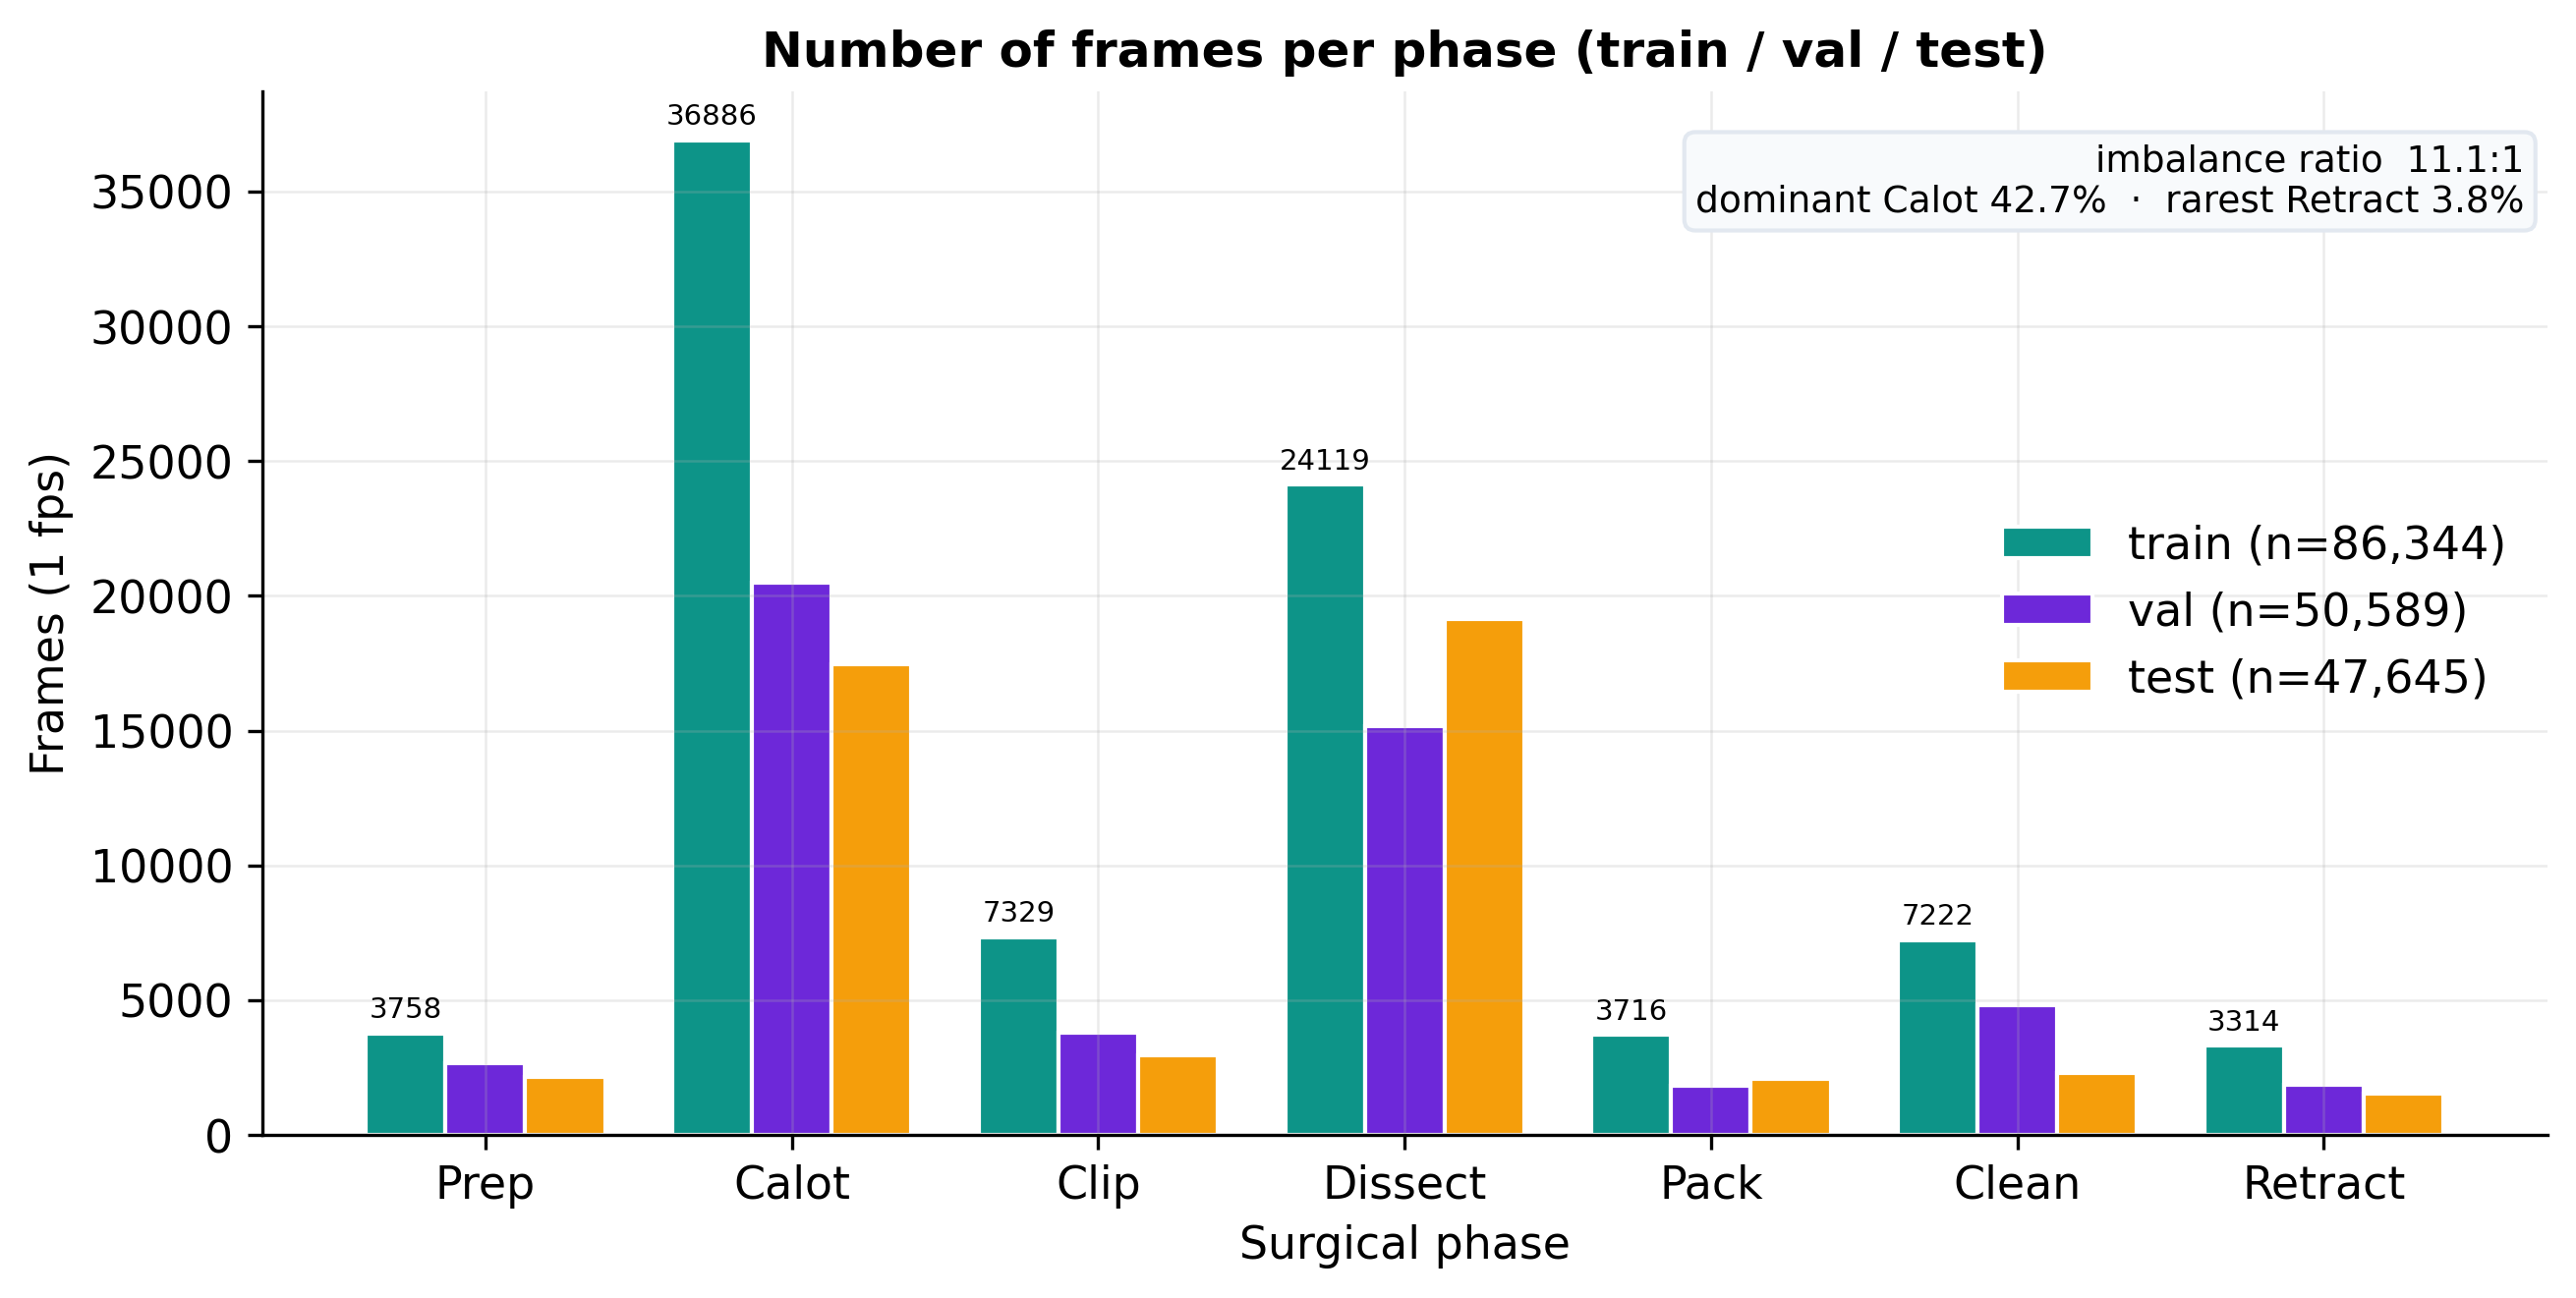
\includegraphics[width=\textwidth]{figures/class_distribution.png}
\caption{Số khung hình của mỗi pha trong các tập huấn luyện, kiểm định và kiểm tra. Các pha phổ biến (Calot, Bóc tách) chiếm ưu thế, còn các pha kết thúc (Đóng gói, Lấy ra) thì hiếm; tỷ lệ này tương tự nhau giữa các tập.}
\label{fig:vn_class_distribution}
\end{figure}

\section{Các Kiến trúc Mô hình}

Ba kiến trúc được so sánh, gọi là M1, M2 và M3. Cả ba có cùng cấu trúc tổng thể, minh họa trong Hình~\ref{fig:vn_transfer_learning}: một mạng nền biến mỗi trong tám khung hình thành một vec-tơ đặc trưng, một mô hình theo thời gian đọc chuỗi tám vec-tơ, và hai lớp đầu ra nhỏ dự đoán, cho từng khung hình, pha và những dụng cụ đang hiện diện. Tất cả mạng nền đều khởi tạo từ trọng số huấn luyện sẵn trên ImageNet, nạp qua thư viện \texttt{timm}.

\begin{figure}[H]
\centering
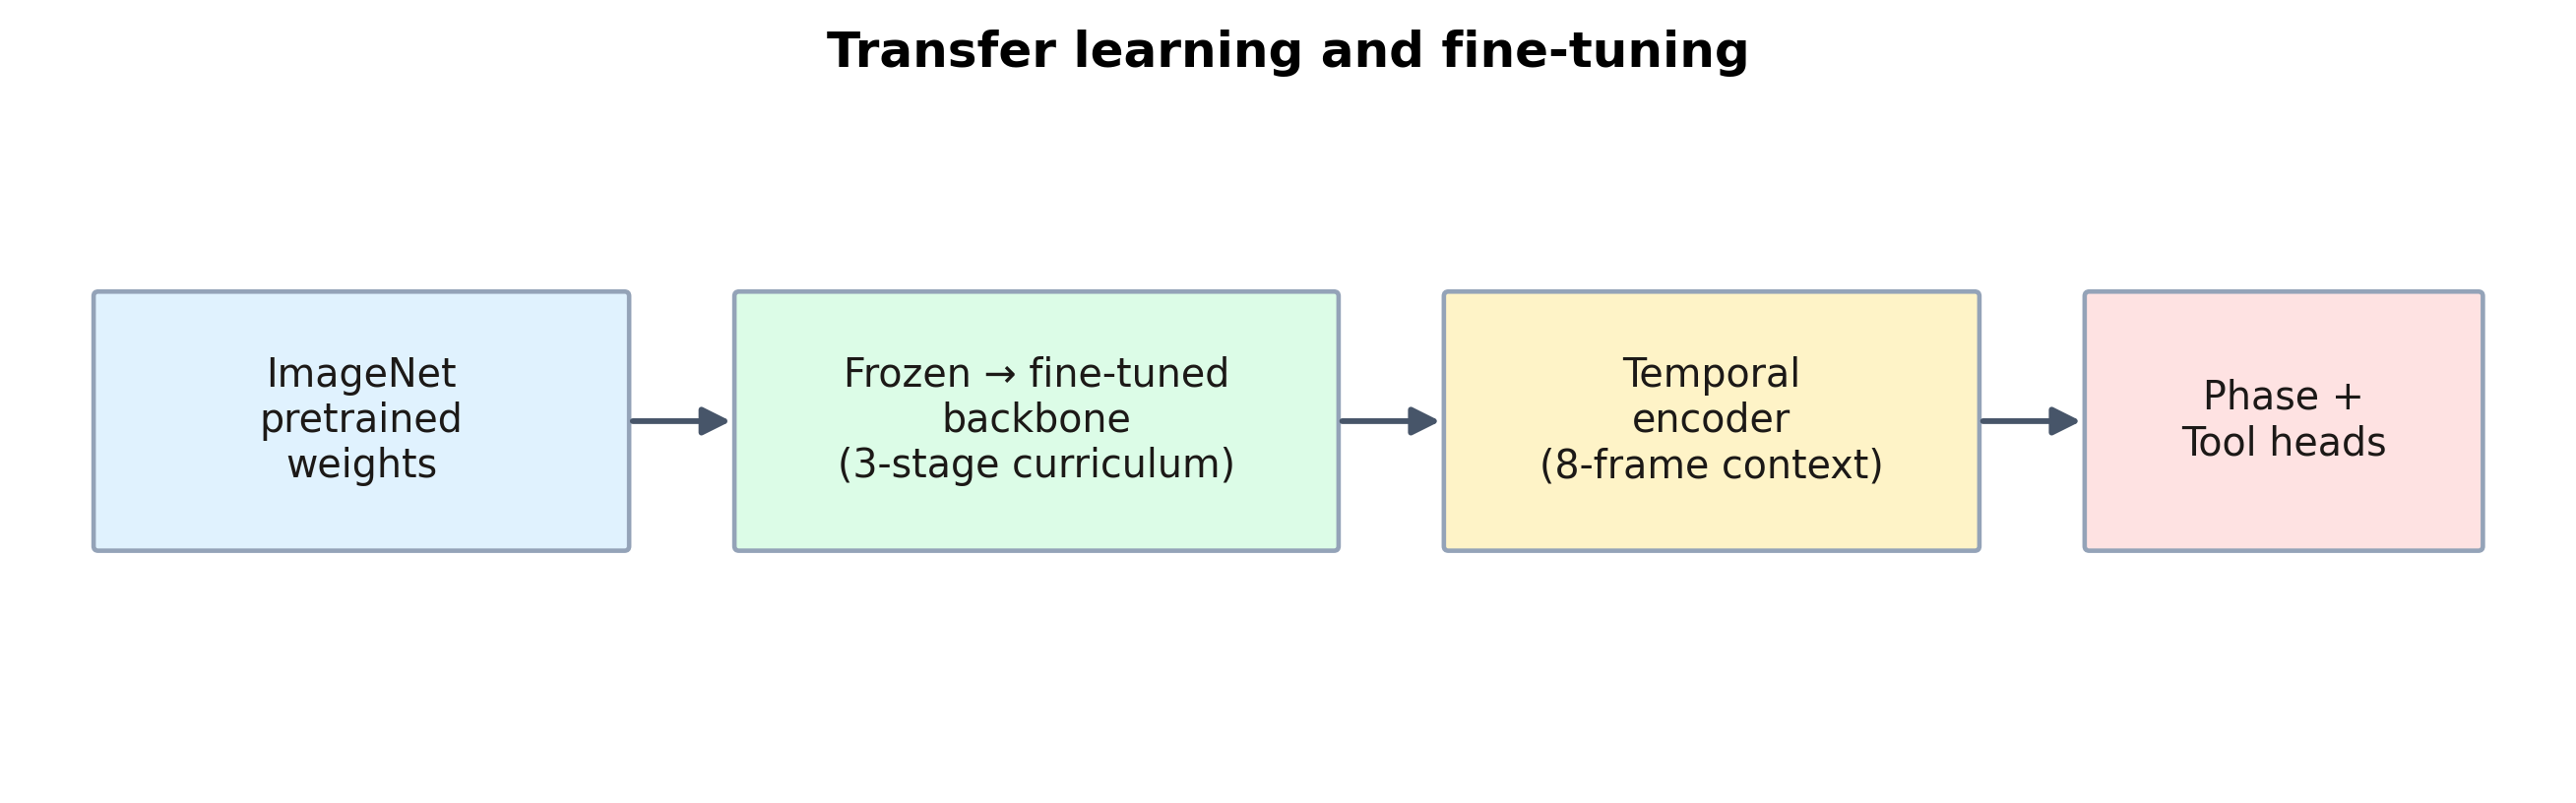
\includegraphics[width=\textwidth]{figures/transfer_learning.png}
\caption{Học chuyển giao (transfer learning) và tinh chỉnh. Mạng nền khởi đầu từ trọng số ImageNet và được tinh chỉnh qua ba giai đoạn; một mô hình theo thời gian gồm tám khung hình bổ sung ngữ cảnh; hai lớp đầu ra dự đoán pha và dụng cụ.}
\label{fig:vn_transfer_learning}
\end{figure}

\subsection{M1 --- ResNet-50 + LSTM hai chiều}

Mạng nền là ResNet-50 với trọng số ImageNet, cho các đặc trưng 2048 chiều. Mô hình theo thời gian là một LSTM hai chiều hai lớp với kích thước ẩn 512. Số tham số huấn luyện: 35,7~M. Cấu hình này theo SV-RCNet.

\subsection{M2 --- EfficientNet-B3 + Mạng tích chập theo thời gian}

Mạng nền là EfficientNet-B3 (đầu ra 1536 chiều). Mô hình theo thời gian là một mạng tích chập theo thời gian hai giai đoạn với tám lớp giãn nở mỗi giai đoạn và 64 bộ lọc, một phiên bản nhỏ hơn của TeCNO để vừa với giới hạn bộ nhớ. Số tham số huấn luyện: 11,2~M.

\subsection{M3 --- Swin-Tiny + Transformer}

Mạng nền là Swin Transformer-Tiny (đầu ra 768 chiều). Mô hình theo thời gian là một bộ mã hóa Transformer ba lớp với sáu đầu (head), kích thước mô hình 384 và kích thước lớp truyền thẳng 768 --- được giữ nhỏ một cách có chủ ý để vừa với giới hạn 4~GB. Số tham số huấn luyện: 31,6~M.

Ở cả ba mô hình, một lớp dropout 0,3 được đặt giữa mô hình theo thời gian và các lớp đầu ra. Lớp đầu ra pha là một lớp tuyến tính cho bảy điểm số; lớp đầu ra dụng cụ cho bảy giá trị sigmoid độc lập.

\begin{table}[H]
\centering
\caption{Tóm tắt ba kiến trúc được đánh giá.}
\label{tab:vn_architectures}
\begin{tabular}{lllrl}
\toprule
\textbf{Mô hình} & \textbf{Mạng nền} & \textbf{Mô hình thời gian} & \textbf{Tham số (M)} & \textbf{Họ} \\
\midrule
M1 & ResNet-50      & LSTM hai chiều       & 35,7 & CNN + RNN \\
M2 & EfficientNet-B3 & TCN nhiều giai đoạn  & 11,2 & CNN + TCN \\
M3 & Swin-Tiny      & Bộ mã hóa Transformer & 31,6 & ViT + Chú ý \\
\bottomrule
\end{tabular}
\end{table}

\section{Pipeline Huấn luyện}

Pipeline huấn luyện được thiết kế xoay quanh sự mất cân bằng 11:1. Nó xử lý vấn đề theo bốn cách --- đánh trọng số lớp, làm mượt nhãn, nhiệm vụ dụng cụ phụ, và một lịch trình theo giai đoạn --- và nghiên cứu loại bỏ (Mục~\ref{sec:vn_ablation}) đo lường mức đóng góp của từng cách. Hình~\ref{fig:vn_training_pipeline} cho cái nhìn tổng quan.

\begin{figure}[H]
\centering
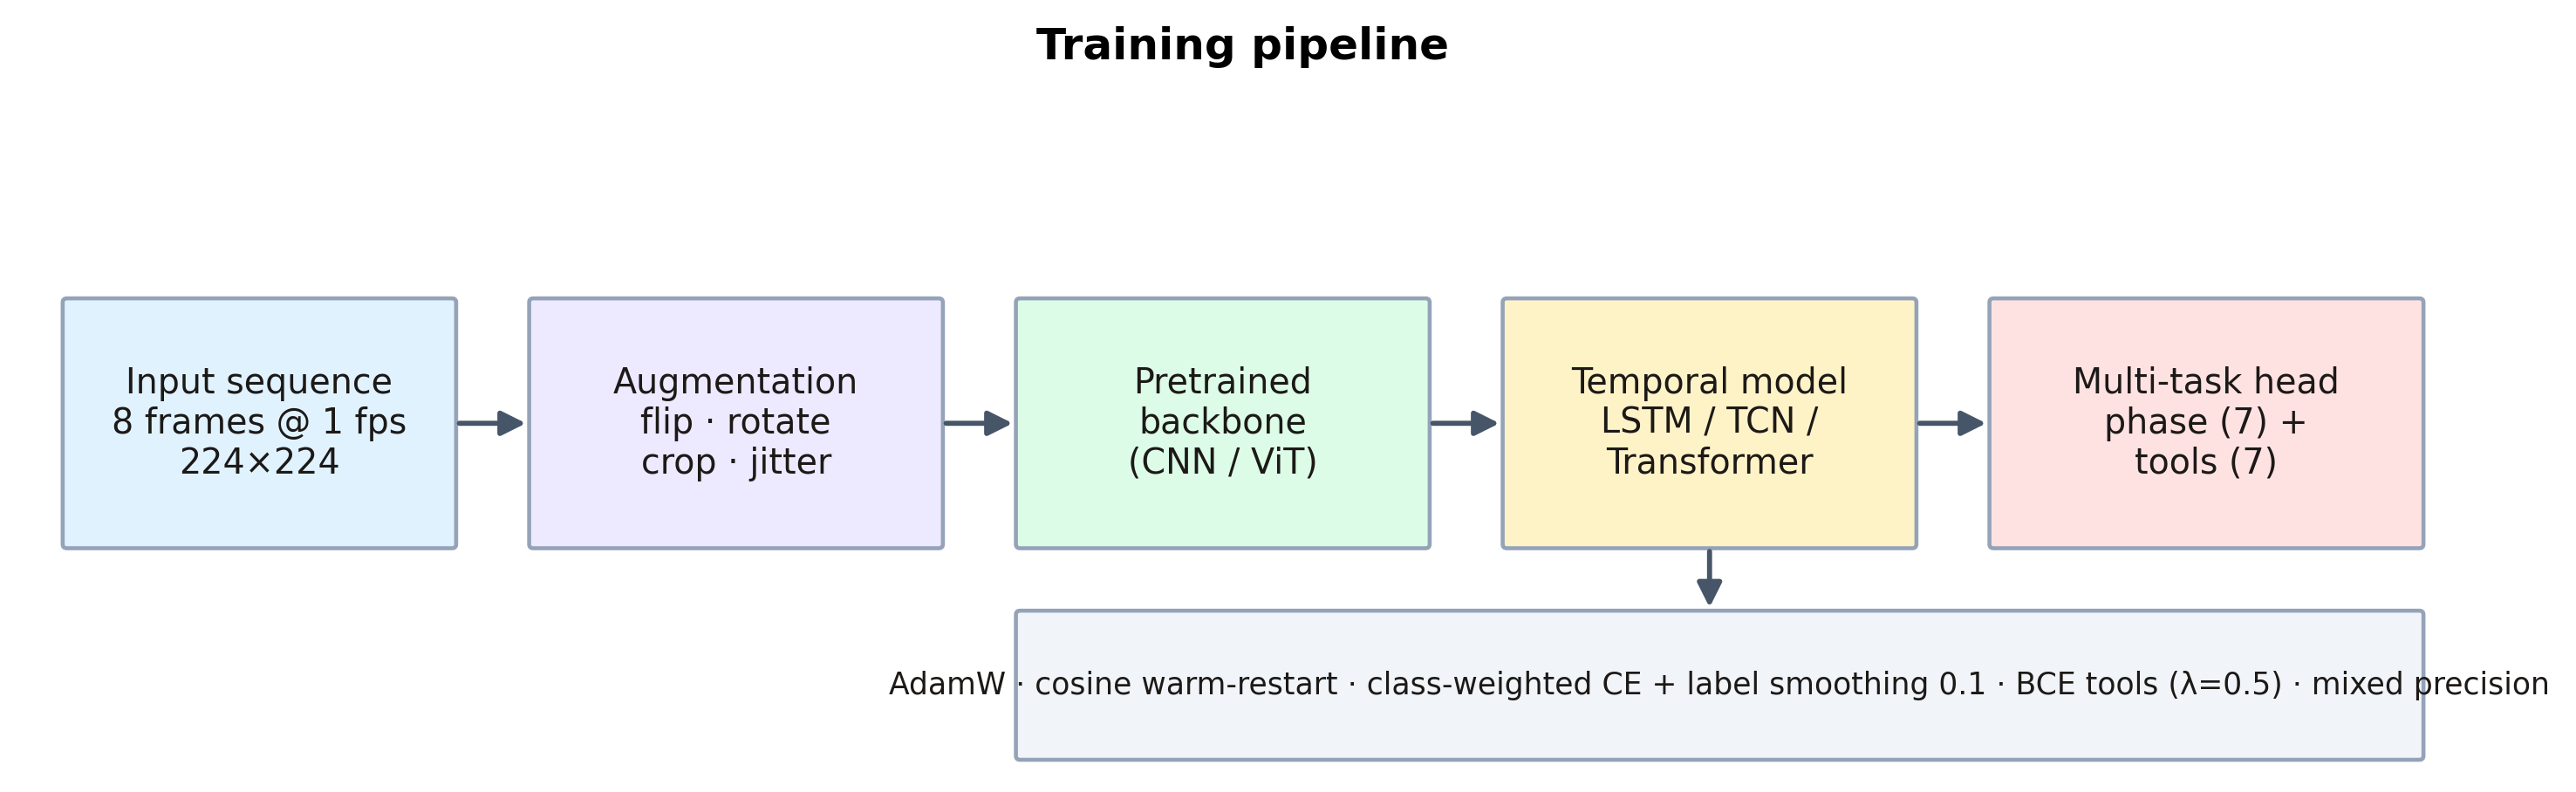
\includegraphics[width=\textwidth]{figures/training_pipeline.png}
\caption{Tổng quan pipeline huấn luyện. Một chuỗi tám khung hình được tăng cường, đi qua mạng nền và mô hình theo thời gian, rồi được phân loại bởi các lớp đầu ra. Huấn luyện dùng AdamW với lịch trình cosine, hàm cross-entropy có trọng số lớp kèm làm mượt nhãn cho pha, và cross-entropy nhị phân cho dụng cụ.}
\label{fig:vn_training_pipeline}
\end{figure}

\subsection{Hàm Mất mát}

Tổng mất mát là tổng có trọng số của một thành phần pha và một thành phần dụng cụ:
\begin{equation}
\mathcal{L} = \mathcal{L}_{\text{pha}}(z_{\text{pha}}, y_{\text{pha}}) + \lambda \cdot \mathcal{L}_{\text{dụng cụ}}(z_{\text{dụng cụ}}, y_{\text{dụng cụ}})
\label{eq:vn_total_loss}
\end{equation}
trong đó $\mathcal{L}_{\text{pha}}$ là cross-entropy có trọng số lớp kèm làm mượt nhãn 0,1, $\mathcal{L}_{\text{dụng cụ}}$ là cross-entropy nhị phân lấy trung bình trên bảy dụng cụ, và $\lambda = 0{,}5$. Trọng số lớp được tính tự động theo nghịch đảo tần suất lớp trên tập huấn luyện:
\begin{equation}
w_c = \frac{N}{C \cdot n_c}
\label{eq:vn_class_weight}
\end{equation}
trong đó $N$ là tổng số khung hình huấn luyện, $C = 7$ là số pha, và $n_c$ là số khung hình thuộc pha $c$. Các trọng số được co giãn để tổng bằng số lớp. Điều này bù lại mức mất cân bằng $11{,}1\times$ mà không bỏ qua các pha phổ biến.

\subsection{Lịch trình Ba Giai đoạn}

Huấn luyện chạy theo ba giai đoạn. Ở Giai đoạn 1 (5 epoch) mạng nền bị đóng băng và chỉ huấn luyện mô hình theo thời gian và các lớp đầu ra. Giai đoạn 2 (10 epoch) tiếp tục điều này. Ở Giai đoạn 3 (10 epoch) mạng nền được mở băng và toàn mạng được tinh chỉnh, với tốc độ học của mạng nền đặt nhỏ hơn phần còn lại mười lần. Các lần chạy loại bỏ dùng phiên bản ngắn hơn $3/6/6$.

\subsection{Tối ưu hóa}

Bộ tối ưu là AdamW với tốc độ học chính $1\times10^{-4}$, tốc độ học mạng nền $1\times10^{-5}$, suy giảm trọng số $1\times10^{-4}$, và một lịch trình cosine. Huấn luyện độ chính xác hỗn hợp (fp16) giữ bộ nhớ trong giới hạn 4~GB; gradient được cắt về chuẩn tối đa 1,0. Kích thước lô là 4 (M1), 8 (M2) và 4 (M3) --- mức lớn nhất vừa với bộ nhớ. Huấn luyện dừng sớm nếu Macro-F1 kiểm định không cải thiện trong năm epoch.

\subsection{Phần cứng và Phần mềm}

Mọi thí nghiệm chạy trên một GPU laptop NVIDIA GeForce RTX 2050 (4~GB) với CPU Intel Core i7 và 24~GB RAM, trên Windows 11, dùng Python 3.13, PyTorch 2.6 với CUDA 12.4, torchvision, timm, OpenCV và scikit-learn.

\section{Các Chỉ số Đánh giá}

Chỉ riêng độ chính xác là gây hiểu lầm trên Cholec80: một mô hình luôn dự đoán hai pha phổ biến sẽ có điểm cao trong khi bỏ qua các pha kết thúc ngắn. Vì vậy, các chỉ số sau được báo cáo kèm với độ chính xác.

\begin{itemize}
    \item \textbf{Macro-F1.} Trung bình của bảy điểm F1 theo từng pha, cho mọi pha trọng số như nhau bất kể nó phổ biến đến đâu. Đây là chỉ số chính để chọn mô hình.
    \item \textbf{Precision / Recall / F1 theo từng pha.} Trình bày kèm ma trận nhầm lẫn để thấy mỗi mô hình sai ở đâu.
    \item \textbf{Điểm Edit.} Một chỉ số ở mức đoạn, đánh giá chất lượng của \emph{chuỗi} pha dự đoán thay vì từng khung hình riêng lẻ.
    \item \textbf{Sai số hiệu chuẩn kỳ vọng (ECE) và Hàm log hợp lý âm (NLL).} Dùng trong phân tích hiệu chuẩn (Mục~\ref{sec:vn_calibration}).
\end{itemize}

Khi kiểm tra, pha dự đoán cho mỗi khung hình là pha có điểm cao nhất, và một bộ lọc trung vị độ dài mười lăm được chạy trên các dự đoán của mỗi video để loại bỏ các lỗi đơn lẻ một khung.

\section{Giải mã Thời gian thực và Hiệu chuẩn}
\label{sec:vn_decoding}

Ngoài bộ lọc trung vị, khóa luận này thêm vào một lớp giải mã biến các điểm số theo từng khung hình thành một chuỗi pha sạch sẽ, chỉ dùng các khung hình quá khứ và hiện tại, để hệ thống có thể chạy ngay trong lúc mổ.

\subsection{Hiệu chuẩn Nhiệt độ}

Với mỗi mô hình, một con số $T^\star$ (nhiệt độ) được tìm trên tập kiểm định bằng cách cực tiểu hóa hàm log hợp lý âm trên một lưới giá trị. Chia các điểm số cho $T^\star$ trước hàm softmax sẽ làm dịu bớt các dự đoán quá tự tin và hạ thấp ECE mà không thay đổi pha được chọn. Các giá trị ước lượng được là 1,3 (M1), 1,1 (M2) và 1,2 (M3) --- đều lớn hơn 1,0, nghĩa là cả ba mô hình đều quá tự tin.

\subsection{Bảng Chuyển pha Học được}

Một bảng chuyển pha $A$, trong đó $A[i, j]$ là xác suất chuyển từ pha $i$ sang pha $j$ từ giây này sang giây kế tiếp, được dựng từ 40 video huấn luyện bằng cách đếm các chuyển tiếp một bước ở 1~fps (kèm một hằng số làm mượt nhỏ). Bảng này có đường chéo trội mạnh --- xác suất ở lại cùng một pha từ giây này sang giây kế tiếp nằm trong khoảng 0,988 đến 0,999 --- và trọng số ngoài đường chéo nằm ở pha kế tiếp, đúng với trình tự cố định của ca cắt túi mật.

\subsection{Bộ Giải mã Thời gian thực}

Bộ giải mã giữ một điểm số đang chạy $\alpha_t[c]$ cho mỗi pha $c$, bằng điểm tổng tốt nhất của bất kỳ đường đi nào kết thúc ở pha $c$ tại thời điểm $t$. Tại mỗi bước,
\begin{equation}
\alpha_t[c] = \log\,\text{softmax}(z_t / T^\star)[c] + \max_{c'} \big( \alpha_{t-1}[c'] + \log A[c', c] \big),
\label{eq:vn_viterbi}
\end{equation}
và pha dự đoán là pha có $\alpha_t$ cao nhất. Mỗi bước chỉ tốn 49 phép tính cho bảy pha, nên nó chạy nhanh hơn nhiều so với thời gian thực. Các điểm số đã hiệu chuẩn và bảng chuyển pha được cộng với nhau trong không gian log; nếu các điểm số quá nhọn thì bảng bị bỏ qua, đó là lý do cần hiệu chuẩn để bảng phát huy tác dụng.

Bộ giải mã được so sánh với ba phương pháp đối chứng: dự đoán thô, làm mượt trung vị-15, và một lượt \textbf{ngoại tuyến} trên toàn bộ video áp đặt trình tự pha cố định bằng cách dùng các khung hình tương lai. Lượt ngoại tuyến cần toàn bộ video, nên nó là một cận trên chứ không phải một phương pháp chạy được trực tiếp.

\section{Thiết kế Nghiên cứu Loại bỏ và Kết hợp Mô hình}

Bốn nghiên cứu loại bỏ, mỗi nghiên cứu thay đổi đúng một yếu tố so với mô hình cơ sở M1, để xem yếu tố đó đáng giá bao nhiêu: \textbf{A1} bỏ nhiệm vụ phát hiện dụng cụ (chỉ còn pha); \textbf{A2} bỏ đánh trọng số lớp (cross-entropy thường); \textbf{A3} tăng gấp đôi chuỗi lên mười sáu khung hình và giảm một nửa kích thước lô; và \textbf{A4} tắt bộ lọc trung vị khi kiểm tra.

Ba cách kết hợp ba mô hình được thử: \textbf{trung bình đơn giản} các dự đoán của chúng, \textbf{trung bình có trọng số theo F1 kiểm định}, và \textbf{biểu quyết đa số} trên lựa chọn theo từng khung hình của chúng. Cả ba đều đi qua cùng một bộ lọc trung vị trước khi đánh giá. Trung bình có trọng số là
\begin{equation}
\hat{y} = \arg\max_c \sum_{m=1}^{M} \omega_m \, p_m(c \mid x),
\label{eq:vn_ensemble}
\end{equation}
trong đó $M = 3$ là số mô hình, $p_m(c \mid x)$ là xác suất mô hình $m$ gán cho pha $c$, và trọng số $\omega_m$ tỷ lệ với Macro-F1 kiểm định của mô hình $m$.

% ======================= CHƯƠNG 4: THÍ NGHIỆM VÀ KẾT QUẢ ==========================
\chapter{Thí nghiệm và Kết quả}

Mọi thí nghiệm chạy trên GPU 4~GB duy nhất mô tả ở Mục~3.3, với hạt giống ngẫu nhiên cố định bằng 42. Kết quả được báo cáo trên tập kiểm tra giữ riêng gồm hai mươi video (mã 61--80), tập mà không mô hình nào thấy trong lúc huấn luyện hay chọn mô hình.

\section{So sánh Ba Mô hình}

\subsection{Kết quả Tổng thể}

Bảng~\ref{tab:vn_model_comparison} báo cáo độ chính xác và Macro-F1 cho ba mô hình, trước và sau khi làm mượt trung vị.

\begin{table}[H]
\centering
\caption{Kết quả trên tập kiểm tra cho ba mô hình. Giá trị tốt nhất in \textbf{đậm}.}
\label{tab:vn_model_comparison}
\begin{tabular}{lcccc}
\toprule
\textbf{Mô hình} & \textbf{Acc. thô} & \textbf{Macro-F1 thô} & \textbf{Acc. mượt} & \textbf{Macro-F1 mượt} \\
\midrule
M1 --- ResNet-50 + BiLSTM      & 0,832 & 0,775 & 0,837 & 0,781 \\
M2 --- EfficientNet-B3 + TCN   & 0,818 & 0,739 & 0,824 & 0,748 \\
\textbf{M3 --- Swin-Tiny + Transformer} & \textbf{0,857} & \textbf{0,807} & \textbf{0,862} & \textbf{0,815} \\
\bottomrule
\end{tabular}
\end{table}

Swin-Transformer M3 tốt nhất trên mọi chỉ số, với Macro-F1 đã làm mượt là \textbf{0,815} --- cao hơn ResNet-LSTM 3,4 điểm và cao hơn EfficientNet-TCN 6,7 điểm. Độ chính xác 0,862 của nó nằm cùng khoảng với Trans-SVNet trên tập dữ liệu này, dù chỉ được huấn luyện trên một GPU laptop 4~GB. Hình~\ref{fig:vn_arch_compare} vẽ điểm số của mỗi mô hình theo số tham số: M3 thắng dù không phải mô hình lớn nhất, và M1 có nhiều tham số hơn nhưng điểm lại thấp hơn, nên kích thước mô hình không phải là yếu tố giới hạn kết quả ở đây.

\begin{figure}[H]
\centering
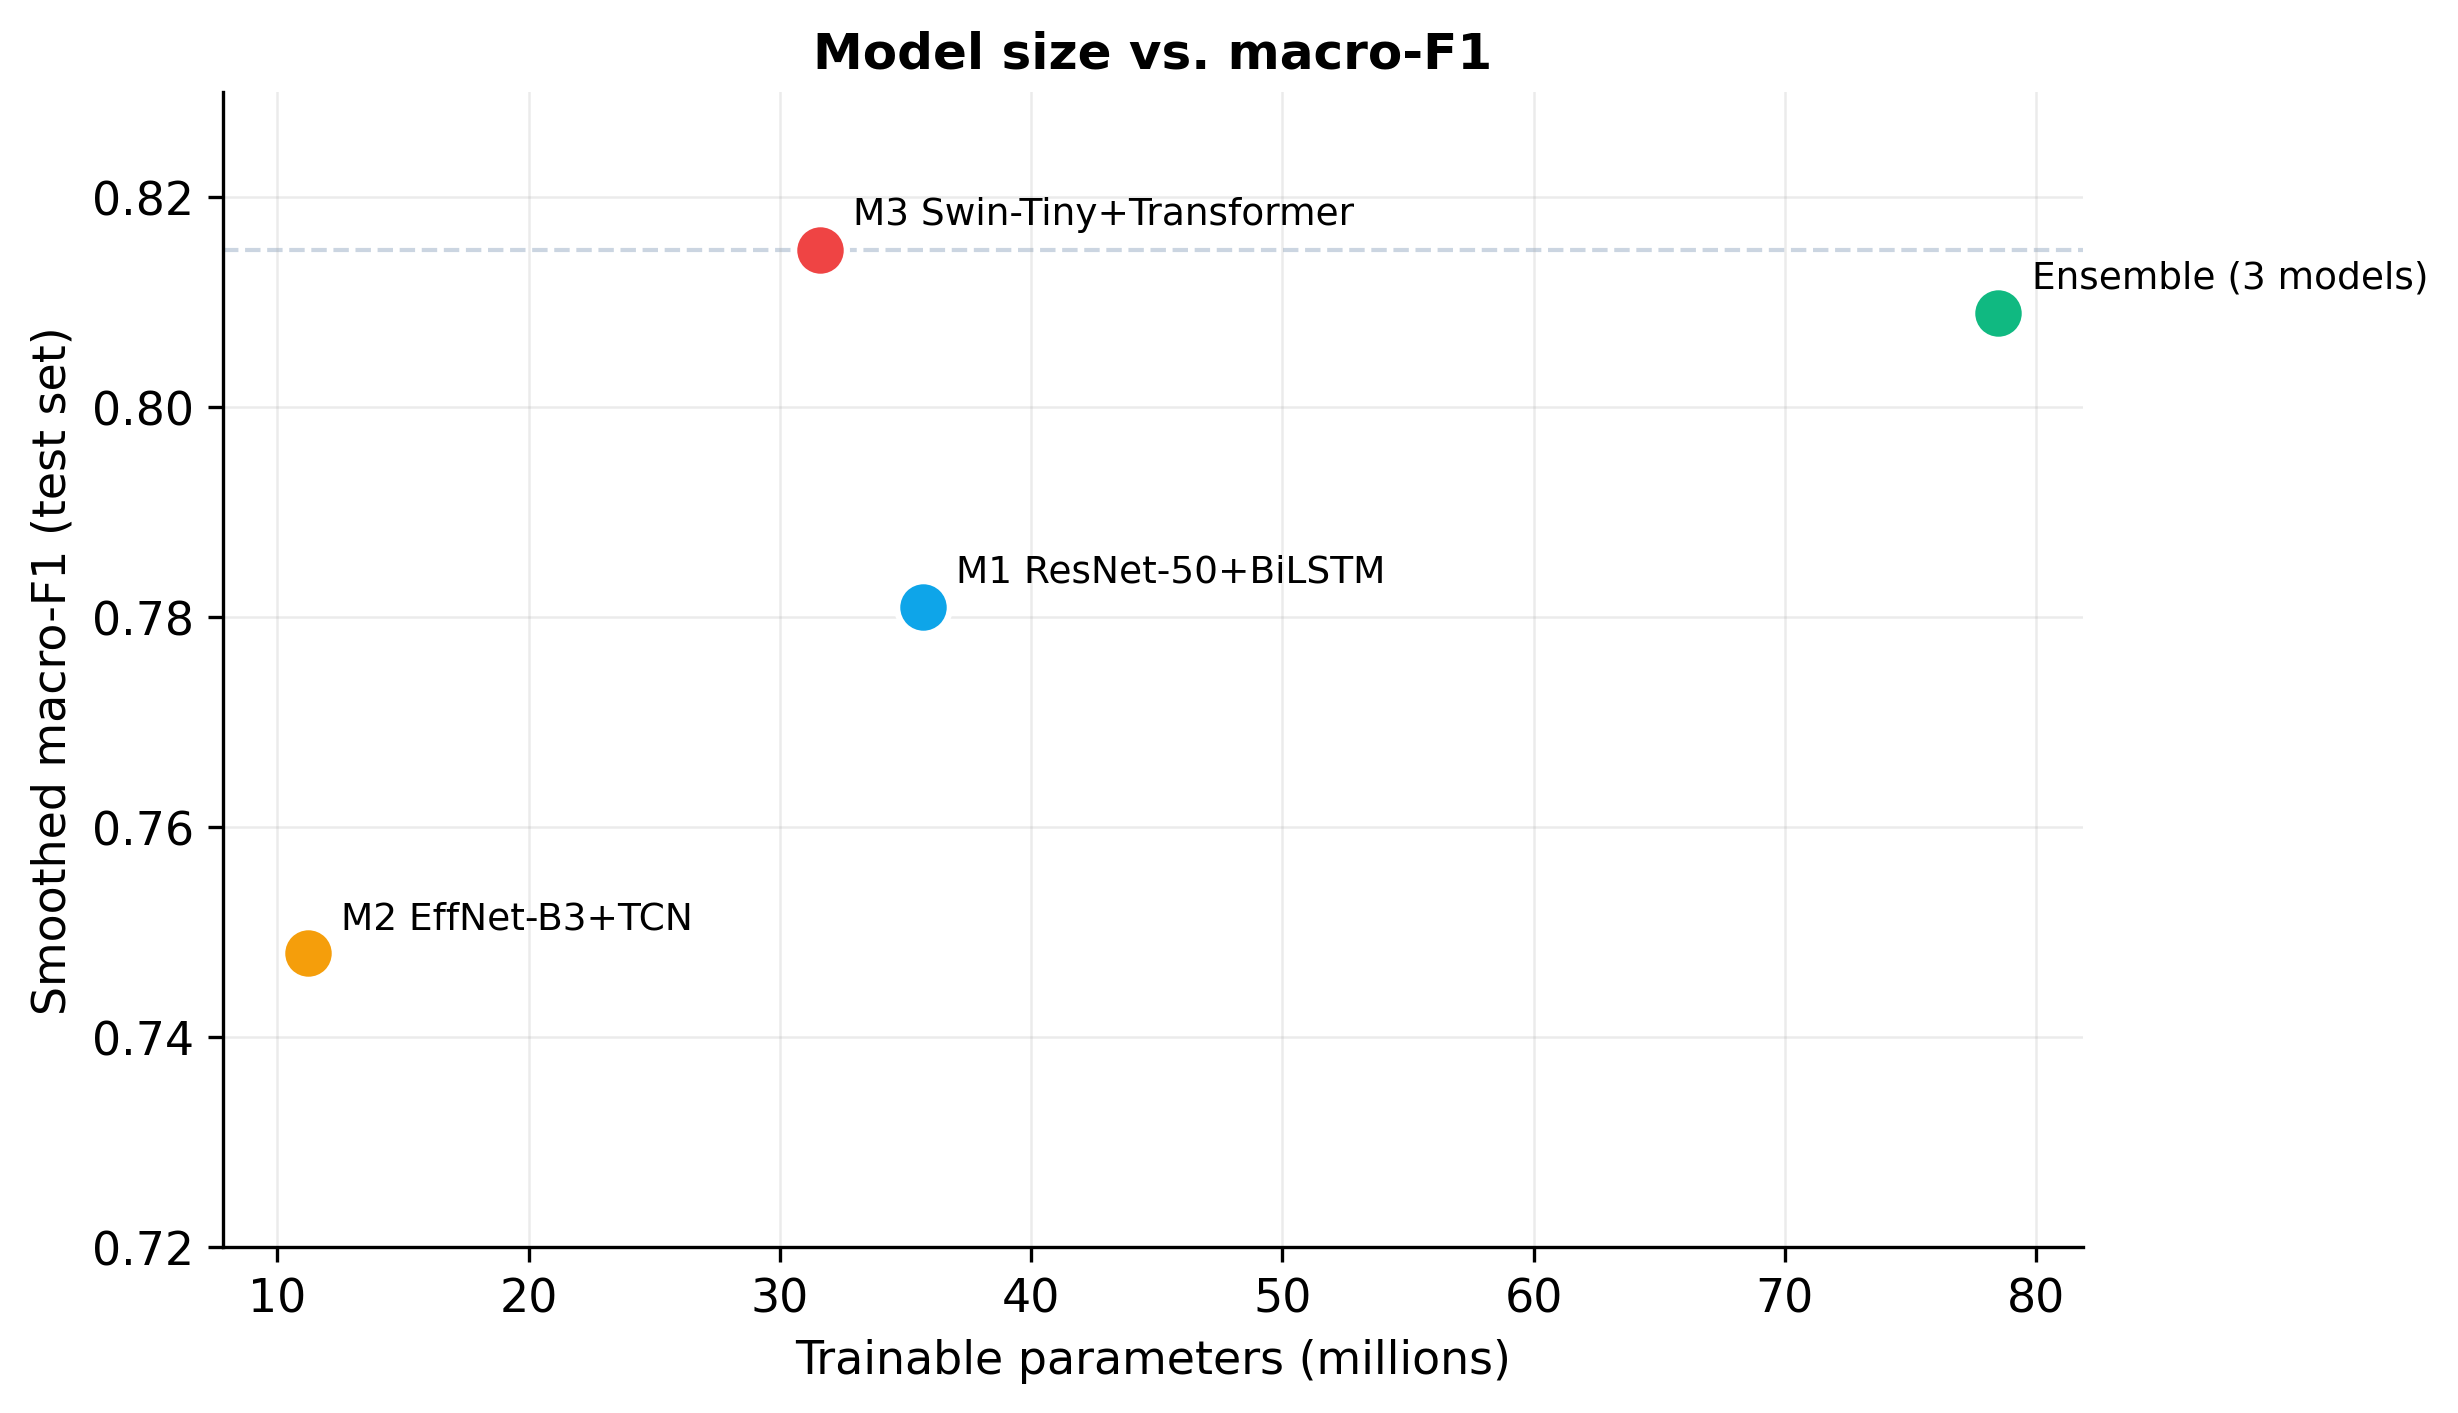
\includegraphics[width=\figwidth]{figures/arch_compare.png}
\caption{Kích thước mô hình so với Macro-F1. Swin-Transformer (M3) đạt điểm cao nhất dù không phải mô hình lớn nhất; EfficientNet-TCN (M2) nhỏ nhất và yếu nhất, một phần vì giai đoạn tinh chỉnh thứ ba của nó bị cắt ngắn do bộ nhớ hạn chế.}
\label{fig:vn_arch_compare}
\end{figure}

\subsection{Diễn biến Huấn luyện}

Hình~\ref{fig:vn_training_history} cho thấy đường cong mất mát và độ chính xác của ba mô hình qua ba giai đoạn. M1 và M3 huấn luyện trơn tru, và độ chính xác kiểm định của chúng tăng vọt ngay khi mạng nền được mở băng ở Giai đoạn 3. Đường của M2 ngắn hơn: với mạng nền EfficientNet-B3 được mở băng, mức dùng bộ nhớ đạt khoảng 97\% giới hạn 4~GB và chỉ một phần Giai đoạn 3 hoàn tất, nên các con số của M2 là cận dưới so với mức nó có thể đạt được nếu có nhiều bộ nhớ hơn.

\begin{figure}[H]
\centering
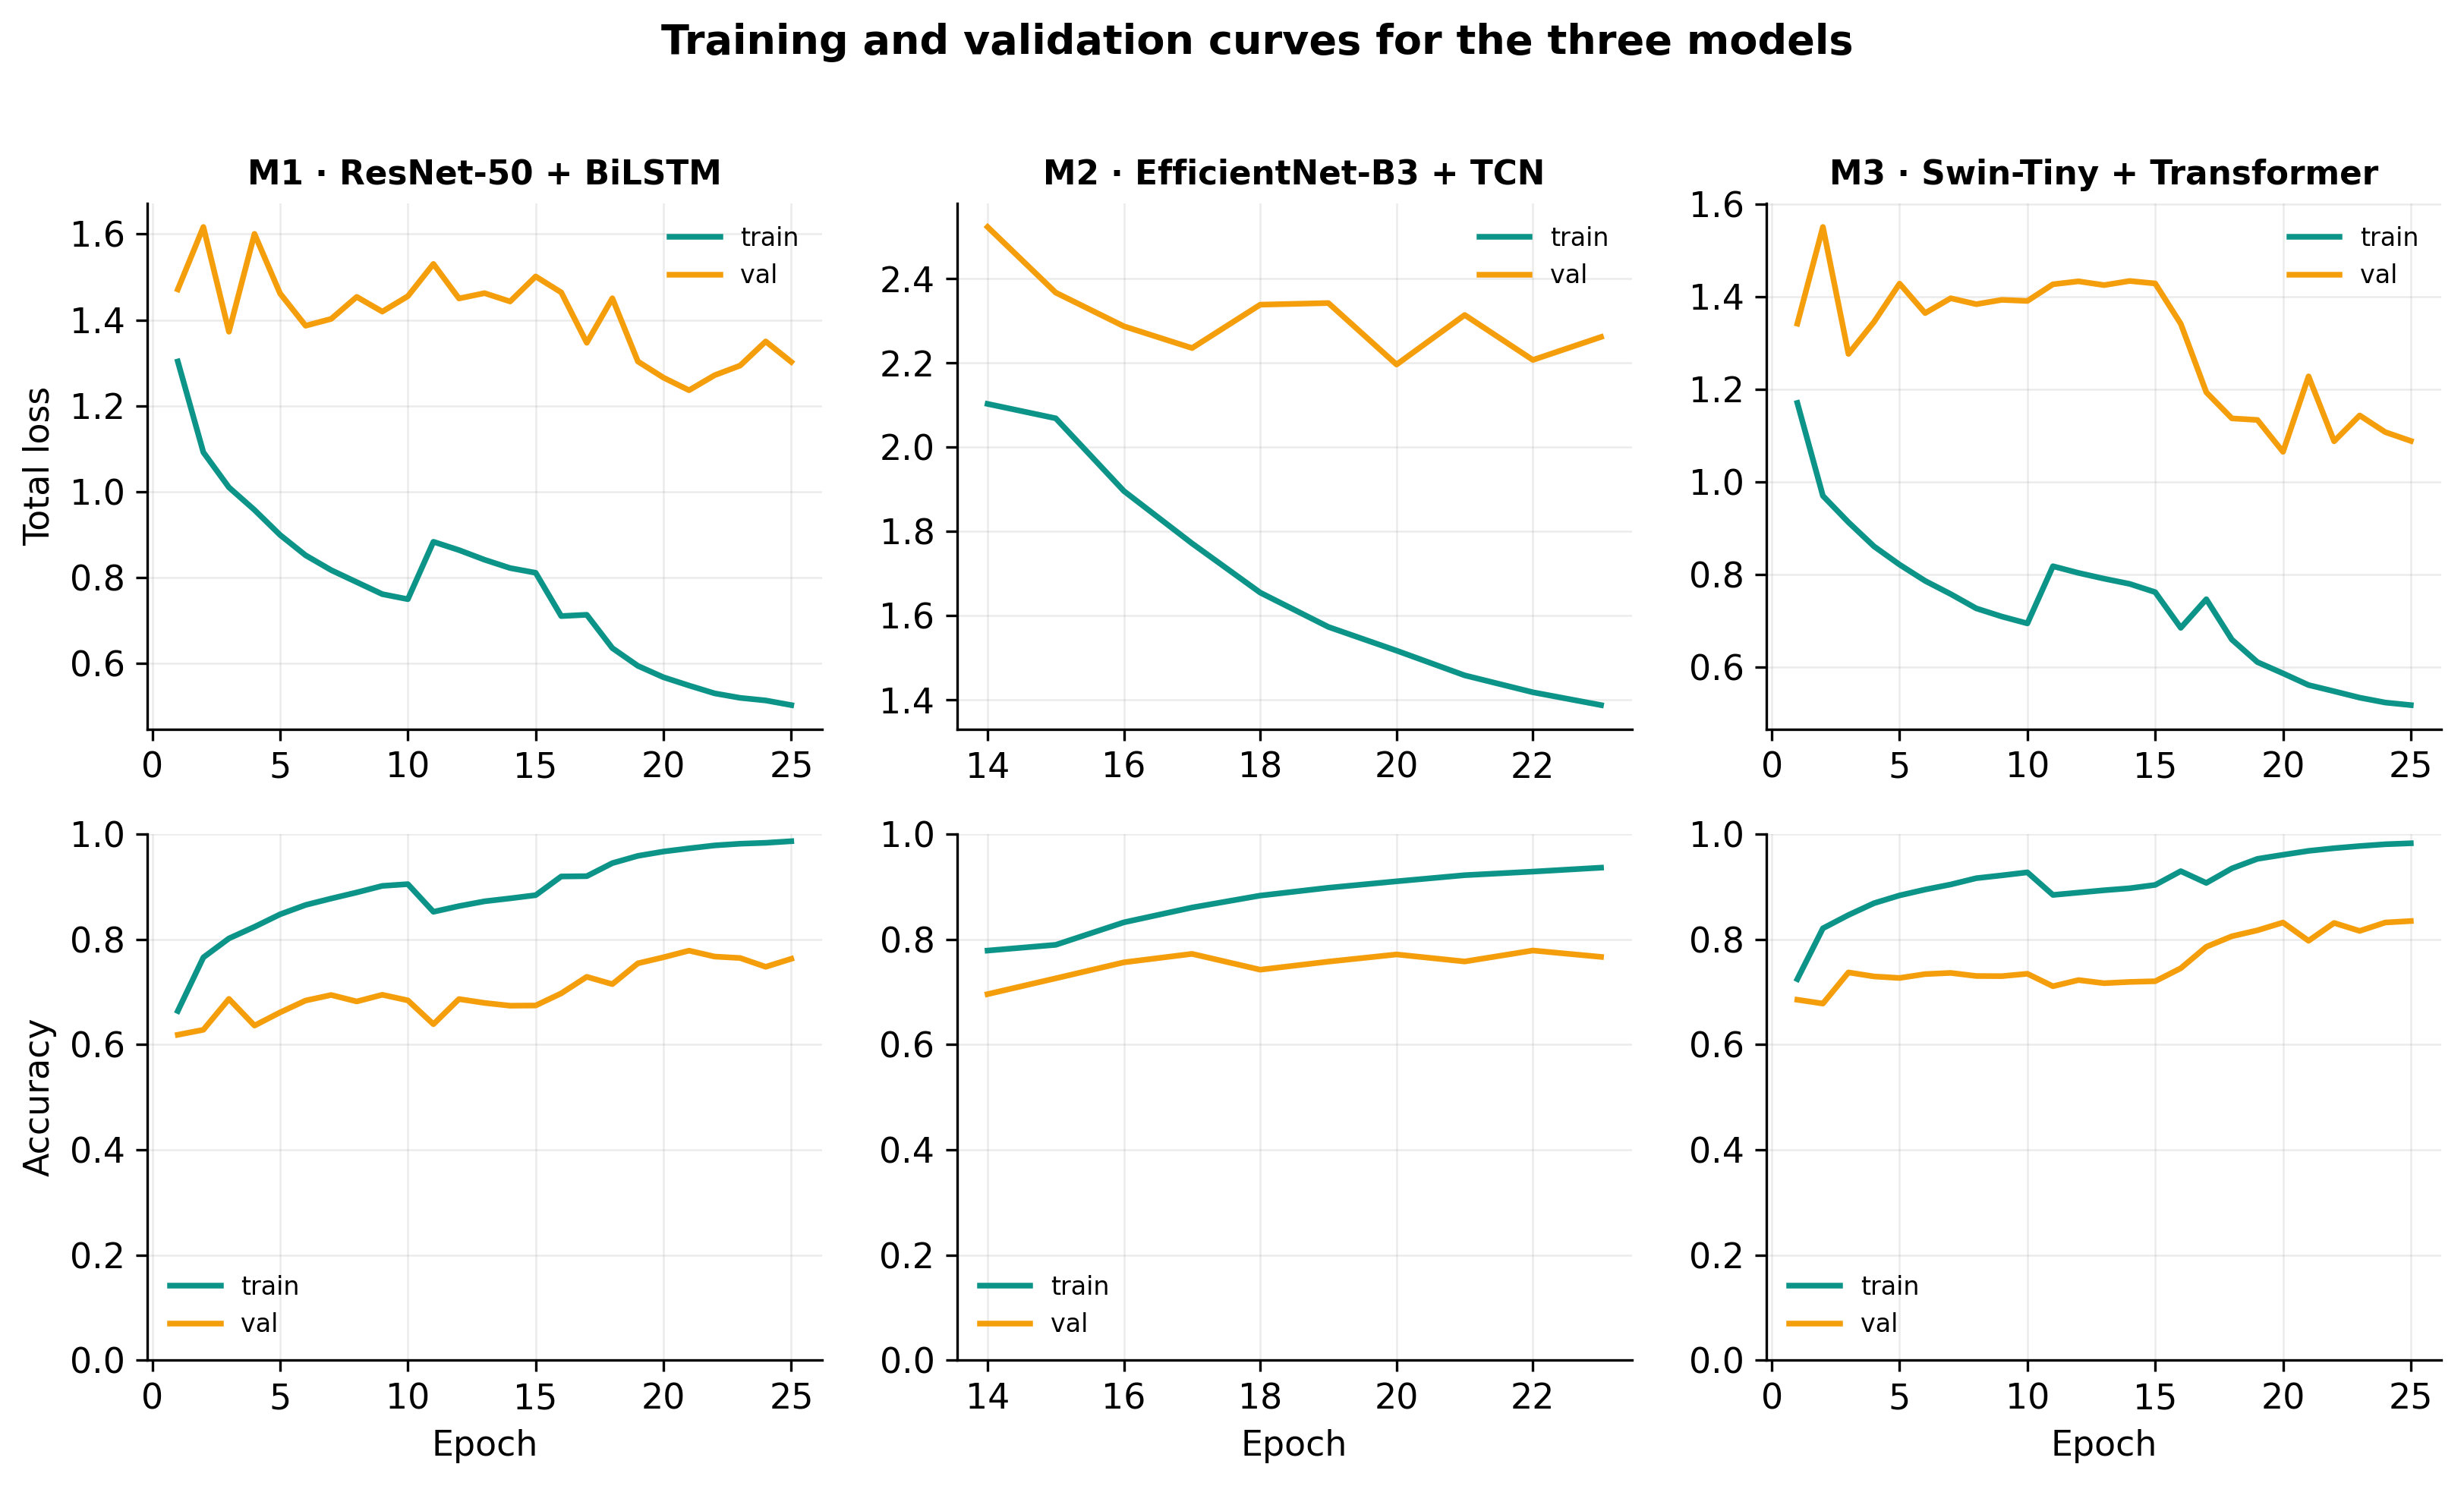
\includegraphics[width=\textwidth]{figures/train_history.png}
\caption{Mất mát và độ chính xác huấn luyện cùng kiểm định qua các epoch cho ba mô hình. M3 cho bước nhảy rõ nhất ở Giai đoạn 3; lần chạy của M2 bị cắt ngắn do bộ nhớ hạn chế khi tinh chỉnh mạng nền.}
\label{fig:vn_training_history}
\end{figure}

\subsection{Phân tích Theo từng Pha}

Bảng~\ref{tab:vn_per_class_m3} trình bày chi tiết precision, recall và F1 theo từng pha cho M3 trên các dự đoán thô của tập kiểm tra.

\begin{table}[H]
\centering
\caption{Precision, recall và F1 theo từng pha cho M3 (dự đoán thô, tập kiểm tra). Pha yếu nhất in \textbf{đậm}.}
\label{tab:vn_per_class_m3}
\begin{tabular}{lccc}
\toprule
\textbf{Pha} & \textbf{Precision} & \textbf{Recall} & \textbf{F1} \\
\midrule
Chuẩn bị                 & 0,830 & 0,803 & 0,816 \\
Bóc tách tam giác Calot  & 0,880 & 0,895 & 0,887 \\
Kẹp và cắt               & 0,815 & 0,796 & 0,806 \\
Bóc tách túi mật         & 0,868 & 0,885 & 0,877 \\
Đóng gói túi mật         & 0,881 & 0,759 & 0,816 \\
Làm sạch và đông máu     & 0,741 & 0,663 & \textbf{0,700} \\
Lấy túi mật ra           & 0,727 & 0,764 & 0,745 \\
\bottomrule
\end{tabular}
\end{table}

Hai pha phổ biến có F1 cao nhất, đúng như mong đợi. Pha yếu nhất là Làm sạch và đông máu (recall 0,663): mô hình thường nhầm việc làm sạch với pha bóc tách xung quanh, điều cũng thấy rõ trong ma trận nhầm lẫn (Hình~\ref{fig:vn_confusion_m3}). Quan trọng là cả bảy pha đều trên F1 $=0{,}70$, nên hàm mất mát có trọng số lớp thực sự ngăn được mô hình sụp về các pha phổ biến.

\begin{figure}[H]
\centering
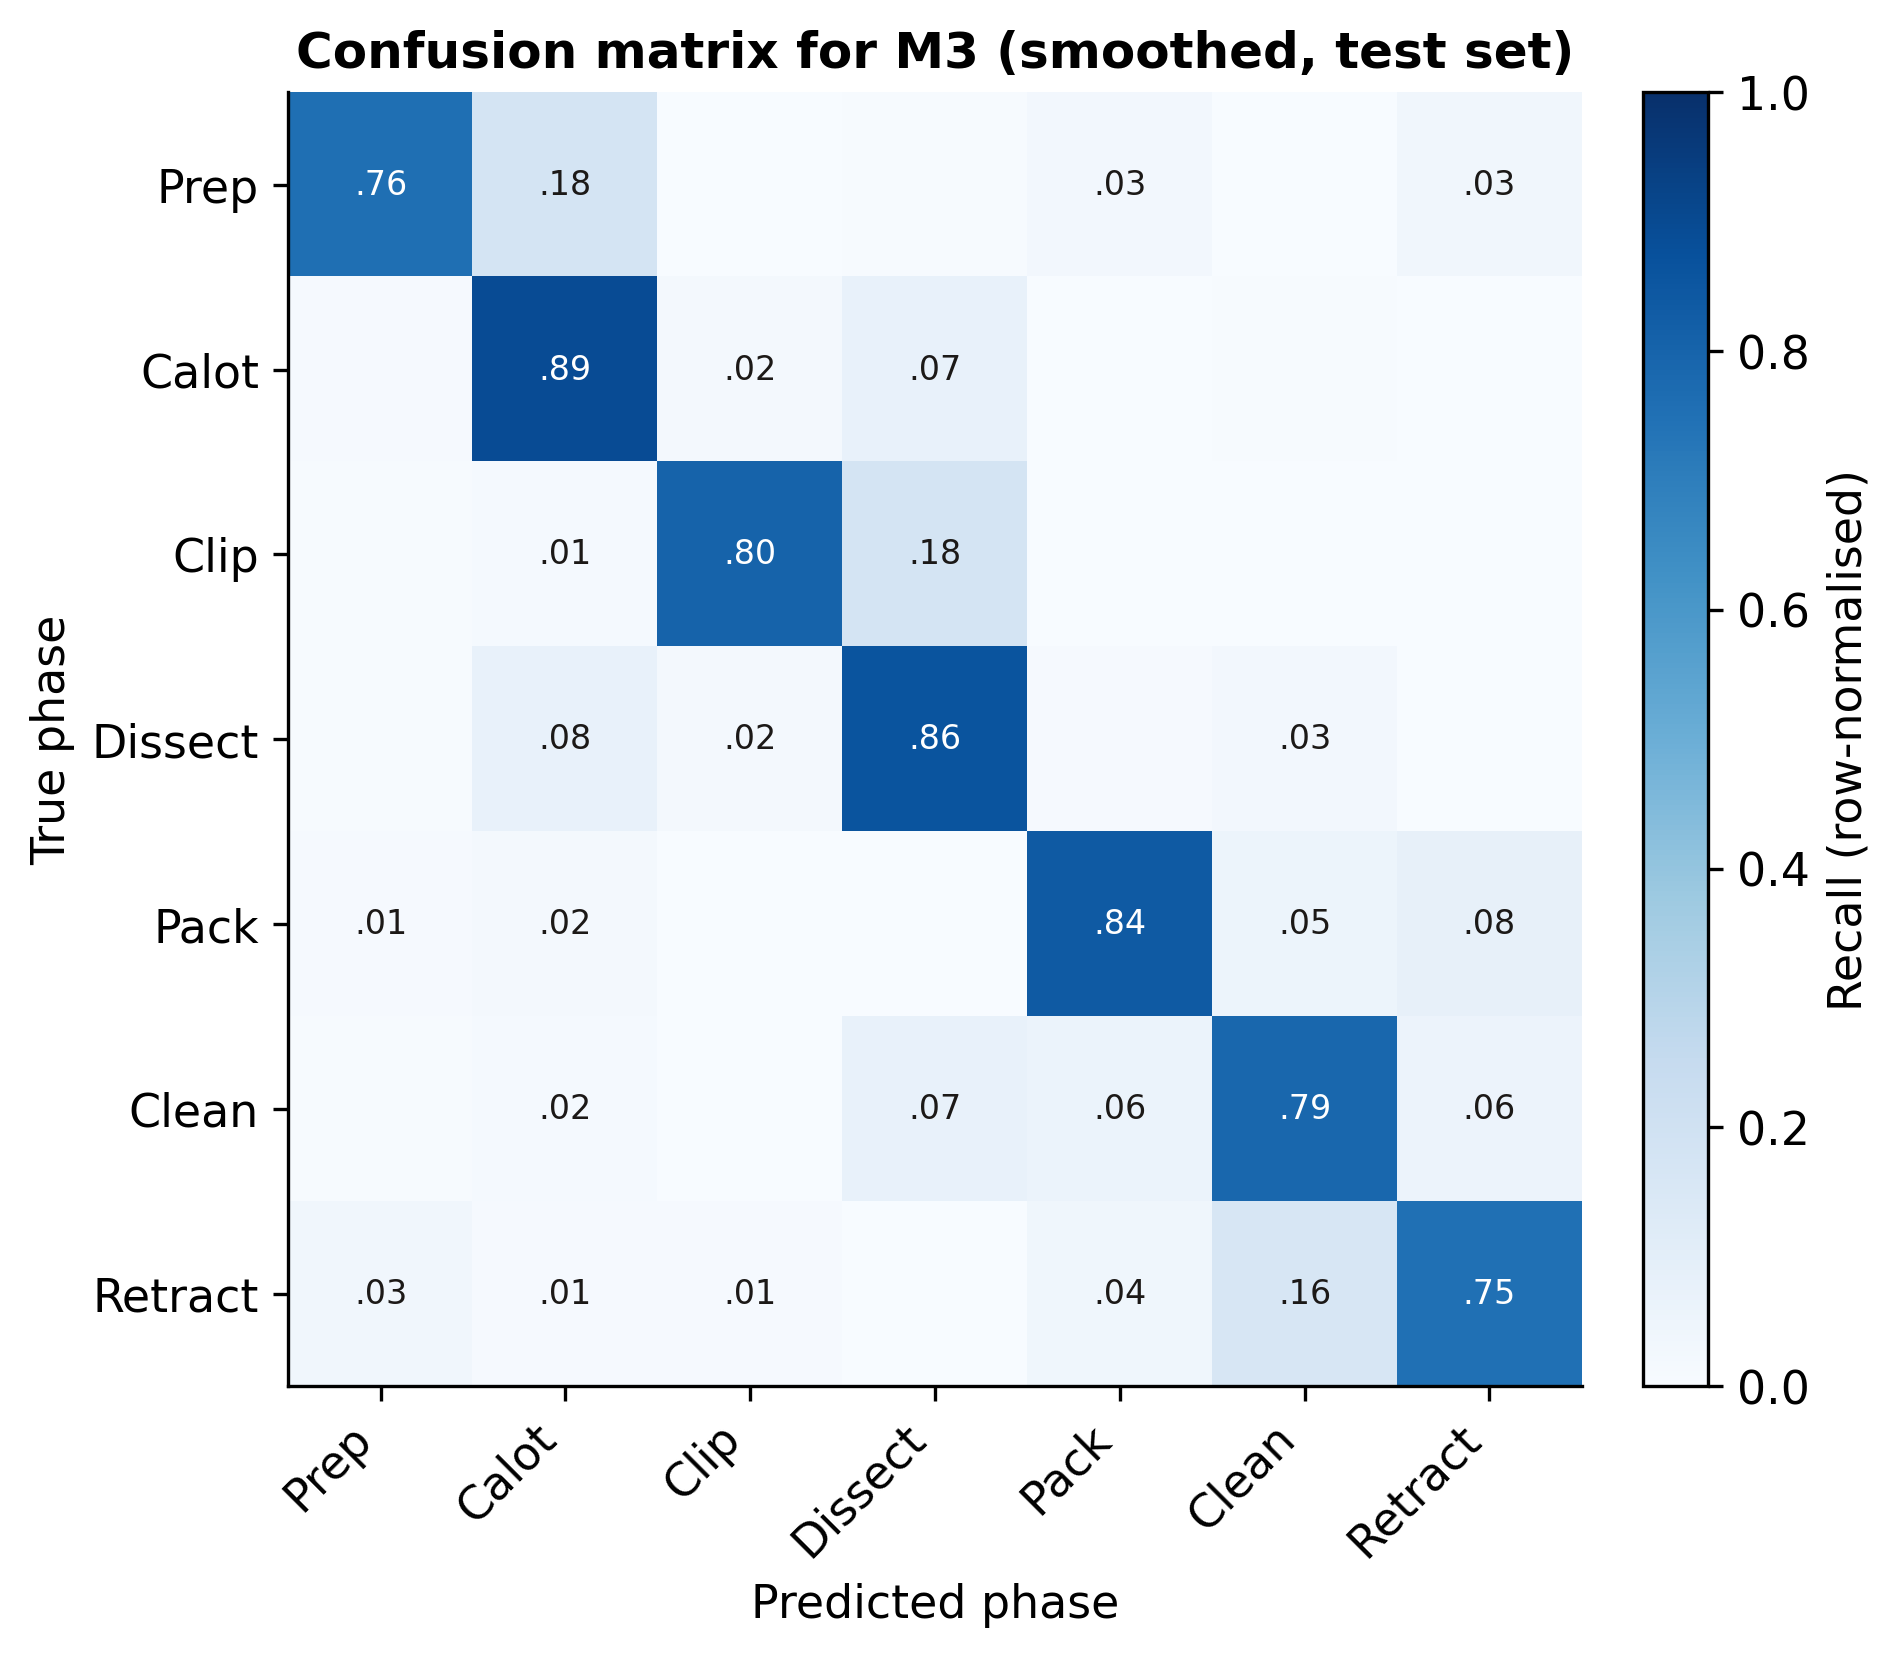
\includegraphics[width=\figwidth]{figures/confusion_m3.png}
\caption{Ma trận nhầm lẫn (mỗi hàng cộng lại bằng 1) cho M3 trên các dự đoán đã làm mượt của tập kiểm tra. Lỗi chính là Làm sạch và Kẹp bị dự đoán thành Bóc tách --- các pha lân cận trông giống nhau --- và không pha nào sụp về các pha phổ biến.}
\label{fig:vn_confusion_m3}
\end{figure}

\section{Nghiên cứu Loại bỏ}
\label{sec:vn_ablation}

Bảng~\ref{tab:vn_ablation} báo cáo bốn nghiên cứu loại bỏ so với mô hình cơ sở M1, tất cả đều huấn luyện với cùng bộ tối ưu và lịch trình ba giai đoạn.

\begin{table}[H]
\centering
\caption{Nghiên cứu loại bỏ (Macro-F1 đã làm mượt trên tập kiểm tra, thay đổi so với M1).}
\label{tab:vn_ablation}
\begin{tabular}{llcc}
\toprule
\textbf{Mã} & \textbf{Thay đổi} & \textbf{Macro-F1 mượt} & \textbf{$\Delta$F1 so với M1}\\
\midrule
\textbf{M1 cơ sở} & cấu hình đầy đủ & \textbf{0,781} & --- \\
\midrule
A1 & bỏ phát hiện dụng cụ (chỉ một nhiệm vụ) & 0,765 & $-1{,}6\%$ \\
A2 & bỏ đánh trọng số lớp                   & 0,761 & $-2{,}0\%$ \\
A3 & chuỗi 16 thay vì 8                     & 0,787 & $+0{,}6\%$ \\
A4 & tắt làm mượt trung vị                  & 0,775 & $-0{,}6\%$ \\
\bottomrule
\end{tabular}
\end{table}

Ba điểm nổi bật. Thứ nhất, bỏ nhiệm vụ dụng cụ (A1) làm mất 1,6 điểm Macro-F1, xác nhận rằng nhiệm vụ phụ này có ích, như EndoNet đã lưu ý đầu tiên. Thứ hai, bỏ đánh trọng số lớp (A2) làm mất 2,0 điểm, nhưng tổn thất không đều: hai pha hiếm nhất --- Lấy túi mật ra và Đóng gói --- mất 5,1 và 2,8 điểm F1 theo pha, trong khi pha phổ biến Calot lại tăng 0,7. Đây đúng là vấn đề mà đánh trọng số lớp được dùng để khắc phục. Thứ ba, A4 cho thấy bộ lọc trung vị làm gì: nó gần như không đổi Macro-F1 ($+0{,}6\%$) nhưng cải thiện điểm edit khoảng 35\%, nên vai trò chính của nó là làm sạch chuỗi pha chứ không phải cải thiện độ chính xác từng khung hình. Tăng gấp đôi độ dài chuỗi (A3) chỉ cho $+0{,}6\%$, nghĩa là cửa sổ tám giây đã bao phủ phần lớn ngữ cảnh hữu ích.

Cộng lại, đánh trọng số lớp và nhiệm vụ dụng cụ đáng giá gần bốn điểm Macro-F1 --- gần bằng khoảng cách 3,4 điểm giữa kiến trúc tốt nhất và kém nhất. Đây là bằng chứng chính cho thấy, trên Cholec80, công thức huấn luyện quan trọng ngang với mạng nền.

\section{Kết quả Kết hợp Mô hình}

Bảng~\ref{tab:vn_ensemble} so sánh ba cách kết hợp các mô hình.

\begin{table}[H]
\centering
\caption{Kết hợp ba mô hình (đã làm mượt, tập kiểm tra). Giá trị tốt nhất in \textbf{đậm}.}
\label{tab:vn_ensemble}
\begin{tabular}{lcc}
\toprule
\textbf{Chiến lược} & \textbf{Độ chính xác} & \textbf{Macro-F1} \\
\midrule
M3 đơn lẻ (mô hình đơn tốt nhất)        & 0,856 & 0,799 \\
Kết hợp --- trung bình softmax đơn giản & 0,863 & 0,808 \\
\textbf{Kết hợp --- trung bình theo F1 kiểm định} & \textbf{0,864} & \textbf{0,809} \\
Kết hợp --- biểu quyết đa số            & 0,857 & 0,799 \\
\bottomrule
\end{tabular}
\end{table}

Trung bình có trọng số theo F1 vượt mô hình đơn tốt nhất 1,0 điểm Macro-F1, với M3 nhận trọng số lớn nhất (0,355), rồi M1 (0,327) và M2 (0,318). Các trọng số gần như bằng nhau, gợi ý rằng ba mô hình đều có năng lực nhưng mắc lỗi tương tự nhau --- chúng có xu hướng sai trên cùng những khung hình khó (thường gần điểm chuyển pha) chứ không phải trên những khung hình khác nhau. Đây là lý do mục tiếp theo chuyển sang giải mã và hiệu chuẩn: nếu các lỗi còn lại tập trung và có cấu trúc, thì một bộ giải mã tốt hơn có thể giúp ích nhiều hơn là thêm mô hình.

\section{Giải mã Thời gian thực và Hiệu chuẩn}
\label{sec:vn_calibration}

Mục này so sánh bộ giải mã thời gian thực ở Mục~\ref{sec:vn_decoding} với các phương pháp đối chứng, dùng cùng các điểm số theo từng khung hình cho mọi phương pháp sao cho mọi khác biệt chỉ đến từ bước giải mã.

\subsection{Hiệu chuẩn}

Bảng~\ref{tab:vn_calibration} báo cáo ECE và NLL trên tập kiểm định trước và sau co giãn nhiệt độ. M1, mô hình quá tự tin nhất, được lợi nhiều nhất --- ECE của nó giảm 66\%. Với cả ba mô hình, nhiệt độ tốt nhất đều lớn hơn 1,0, dấu hiệu của sự quá tự tin. Hình~\ref{fig:vn_reliability} cho thấy các biểu đồ độ tin cậy: độ chính xác thô nằm dưới đường chéo ở các khoảng tin cậy cao, và co giãn nhiệt độ kéo đường cong trở lại về phía đường chéo.

\begin{table}[H]
\centering
\caption{Hiệu chuẩn trên tập kiểm định trước và sau co giãn nhiệt độ. ECE tốt nhất in \textbf{đậm}.}
\label{tab:vn_calibration}
\begin{tabular}{lccccc}
\toprule
\textbf{Mô hình} & \textbf{$T^\star$} & \textbf{ECE thô} & \textbf{ECE hc} & \textbf{NLL thô} & \textbf{NLL hc} \\
\midrule
M1 --- ResNet-LSTM      & 1,30 & 0,109 & \textbf{0,037} & 0,897 & 0,855 \\
M2 --- EffNet-TCN       & 1,10 & 0,059 & 0,074 & 0,824 & 0,817 \\
M3 --- Swin-Transformer & 1,20 & 0,074 & 0,070 & 0,688 & 0,667 \\
\bottomrule
\end{tabular}
\end{table}

\begin{figure}[H]
\centering
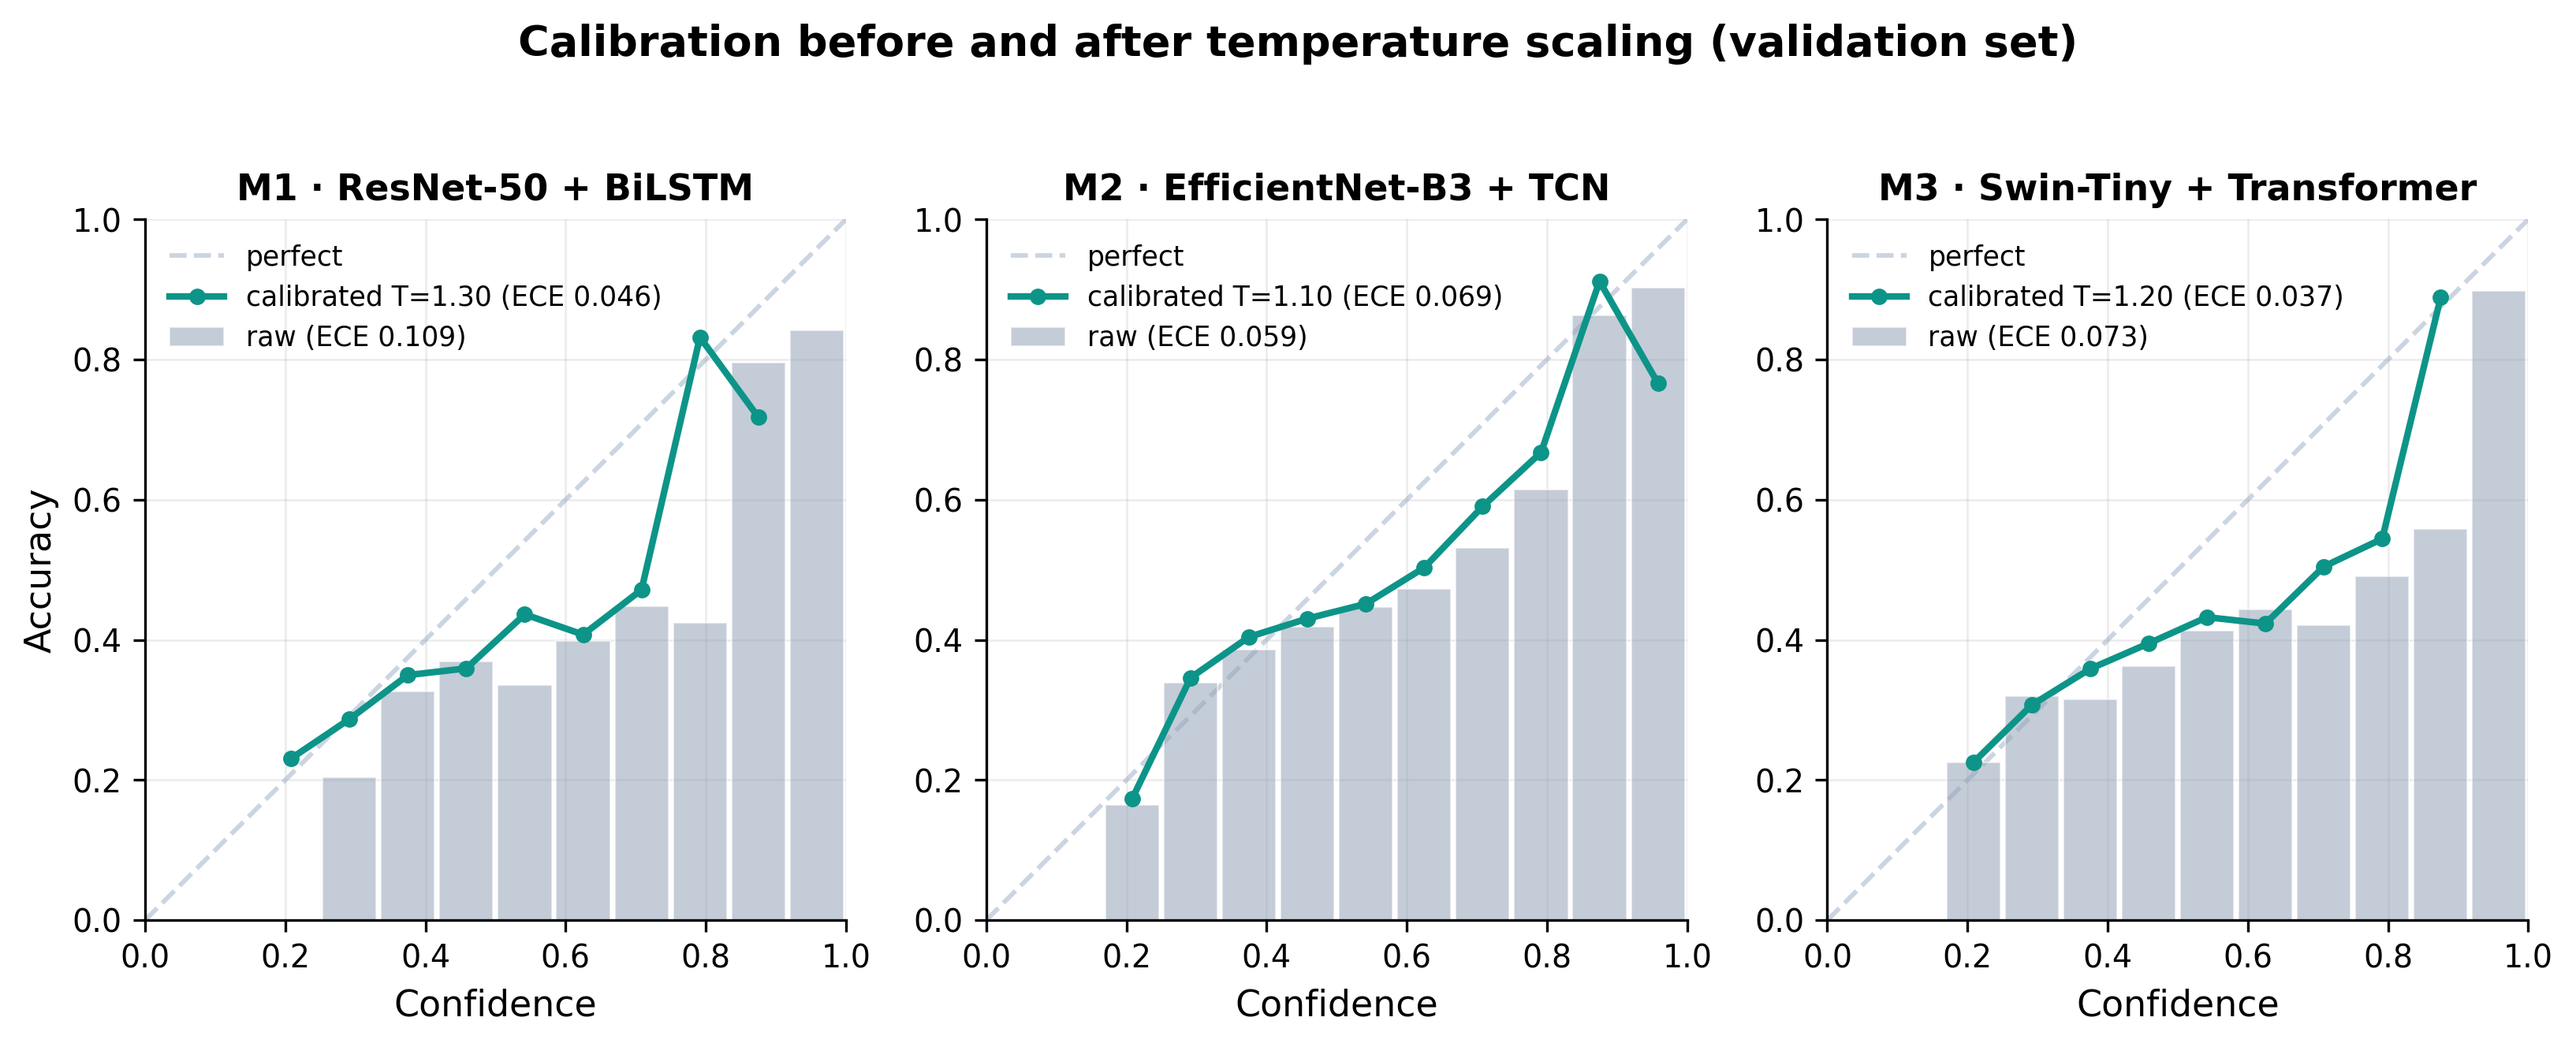
\includegraphics[width=\textwidth]{figures/reliability.png}
\caption{Biểu đồ độ tin cậy trên tập kiểm định. Cột xám là độ chính xác thô trong mỗi khoảng tin cậy; đường màu xanh là sau co giãn nhiệt độ; đường chéo nét đứt là hiệu chuẩn hoàn hảo. M1 dịch về phía đường chéo nhiều nhất.}
\label{fig:vn_reliability}
\end{figure}

\subsection{Đánh giá Bộ Giải mã}

Bảng~\ref{tab:vn_decoder} báo cáo độ chính xác và Macro-F1 trên tập kiểm tra cho mỗi bộ giải mã trên mỗi mô hình. Bộ giải mã được đề xuất (điểm số đã hiệu chuẩn cộng bảng chuyển pha) là bộ giải mã thời gian thực tốt nhất trên cả ba mô hình; bộ giải mã ngoại tuyến chỉ được nêu như một cận trên. Hình~\ref{fig:vn_benchmark} cho thấy cùng so sánh đó.

\begin{table}[H]
\centering
\caption{So sánh bộ giải mã (tập kiểm tra, độ chính xác / Macro-F1). Bộ giải mã ngoại tuyến $\dagger$ dùng các khung hình tương lai và chỉ là cận trên. Giá trị \emph{thời gian thực} tốt nhất in \textbf{đậm}.}
\label{tab:vn_decoder}
\begin{tabular}{lccc}
\toprule
\textbf{Bộ giải mã} & \textbf{M1 Acc / F1} & \textbf{M2 Acc / F1} & \textbf{M3 Acc / F1} \\
\midrule
Dự đoán thô              & 82,4 / 0,763 & 81,2 / 0,738 & 85,3 / 0,794 \\
Lọc trung vị-15          & 82,7 / 0,768 & 81,7 / 0,746 & 85,5 / 0,800 \\
Trình tự cố định + hc    & 82,5 / 0,777 & 82,4 / 0,767 & 86,0 / 0,802 \\
\textbf{Bộ giải mã đề xuất} & \textbf{83,0 / 0,771} & \textbf{82,9 / 0,764} & \textbf{86,0 / 0,806} \\
\midrule
Ngoại tuyến (toàn video) $\dagger$ & 91,8 / 0,859 & 91,8 / 0,849 & 90,1 / 0,832 \\
\bottomrule
\end{tabular}
\end{table}

\begin{figure}[H]
\centering
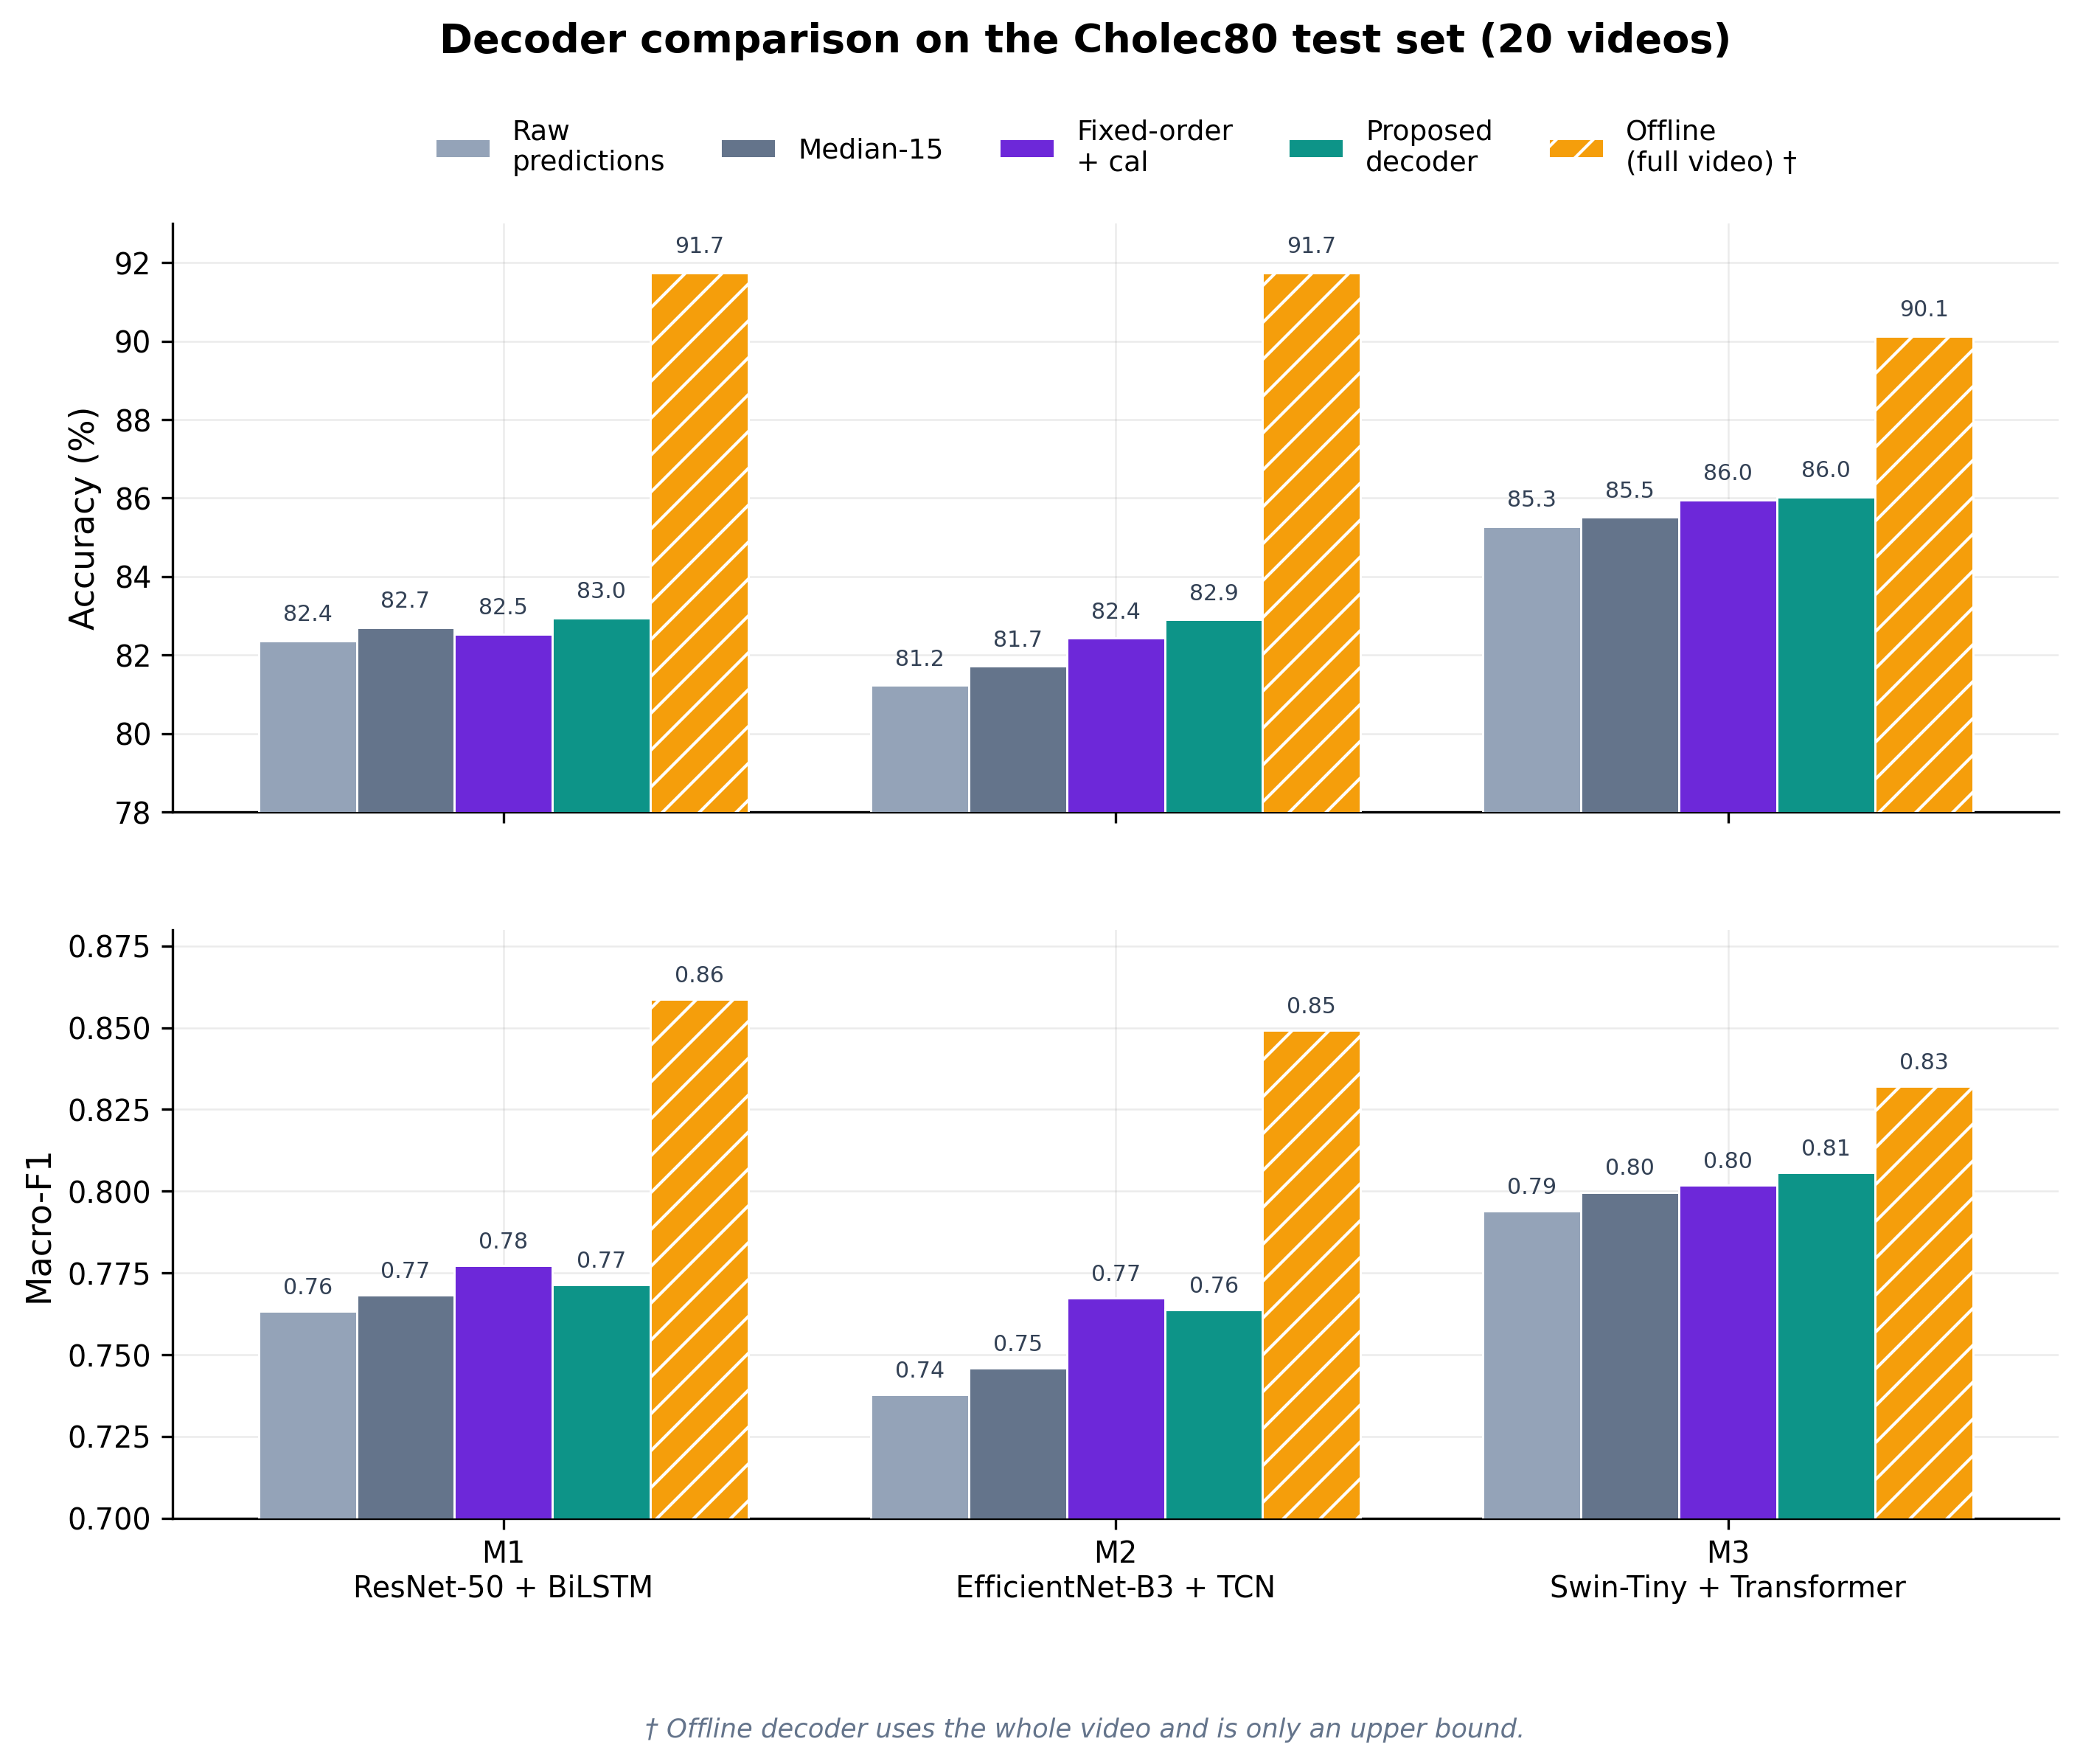
\includegraphics[width=\textwidth]{figures/benchmark.png}
\caption{So sánh bộ giải mã trên tập kiểm tra: độ chính xác và Macro-F1. Bộ giải mã đề xuất (màu xanh) là lựa chọn thời gian thực tốt nhất trên mọi mô hình; bộ giải mã ngoại tuyến (màu hổ phách, gạch chéo) dùng các khung hình tương lai và là cận trên.}
\label{fig:vn_benchmark}
\end{figure}

\subsection{Ý nghĩa Thống kê}

Vì các mức tăng trung bình trông nhỏ, một kiểm định ghép cặp theo từng video là quan trọng. Bảng~\ref{tab:vn_significance} báo cáo kiểm định Wilcoxon ghép cặp và hệ số Cohen $d$ trên hai mươi video kiểm tra, so sánh bộ giải mã đề xuất với dự đoán thô. Cả ba mô hình đều cho một cải thiện rõ ràng và nhất quán ($p < 0{,}001$, $d > 0{,}97$): mức tăng nhỏ về độ lớn nhưng đúng trên mọi video chứ không do một vài ngoại lệ. Bộ giải mã tốn 0,011--0,024~ms mỗi khung hình, thấp hơn nhiều so với 40~ms khả dụng giữa các khung hình trong video 25~fps. Hình~\ref{fig:vn_transition_significance} cho thấy bảng chuyển pha học được và các mức tăng theo từng video cạnh nhau.

\begin{table}[H]
\centering
\caption{Mức cải thiện theo từng video của bộ giải mã đề xuất so với dự đoán thô (20 video kiểm tra).}
\label{tab:vn_significance}
\begin{tabular}{lccc}
\toprule
\textbf{Mô hình} & \textbf{$\Delta$Acc (đpt)} & \textbf{Wilcoxon $p$} & \textbf{Cohen $d$} \\
\midrule
M1 --- ResNet-LSTM      & $+0{,}62$ & $<0{,}0001$ & 1,38 \\
M2 --- EffNet-TCN       & $+1{,}74$ & $0{,}0001$  & 1,25 \\
M3 --- Swin-Transformer & $+0{,}76$ & $0{,}0001$  & 0,98 \\
\bottomrule
\end{tabular}
\end{table}

\begin{figure}[H]
\centering
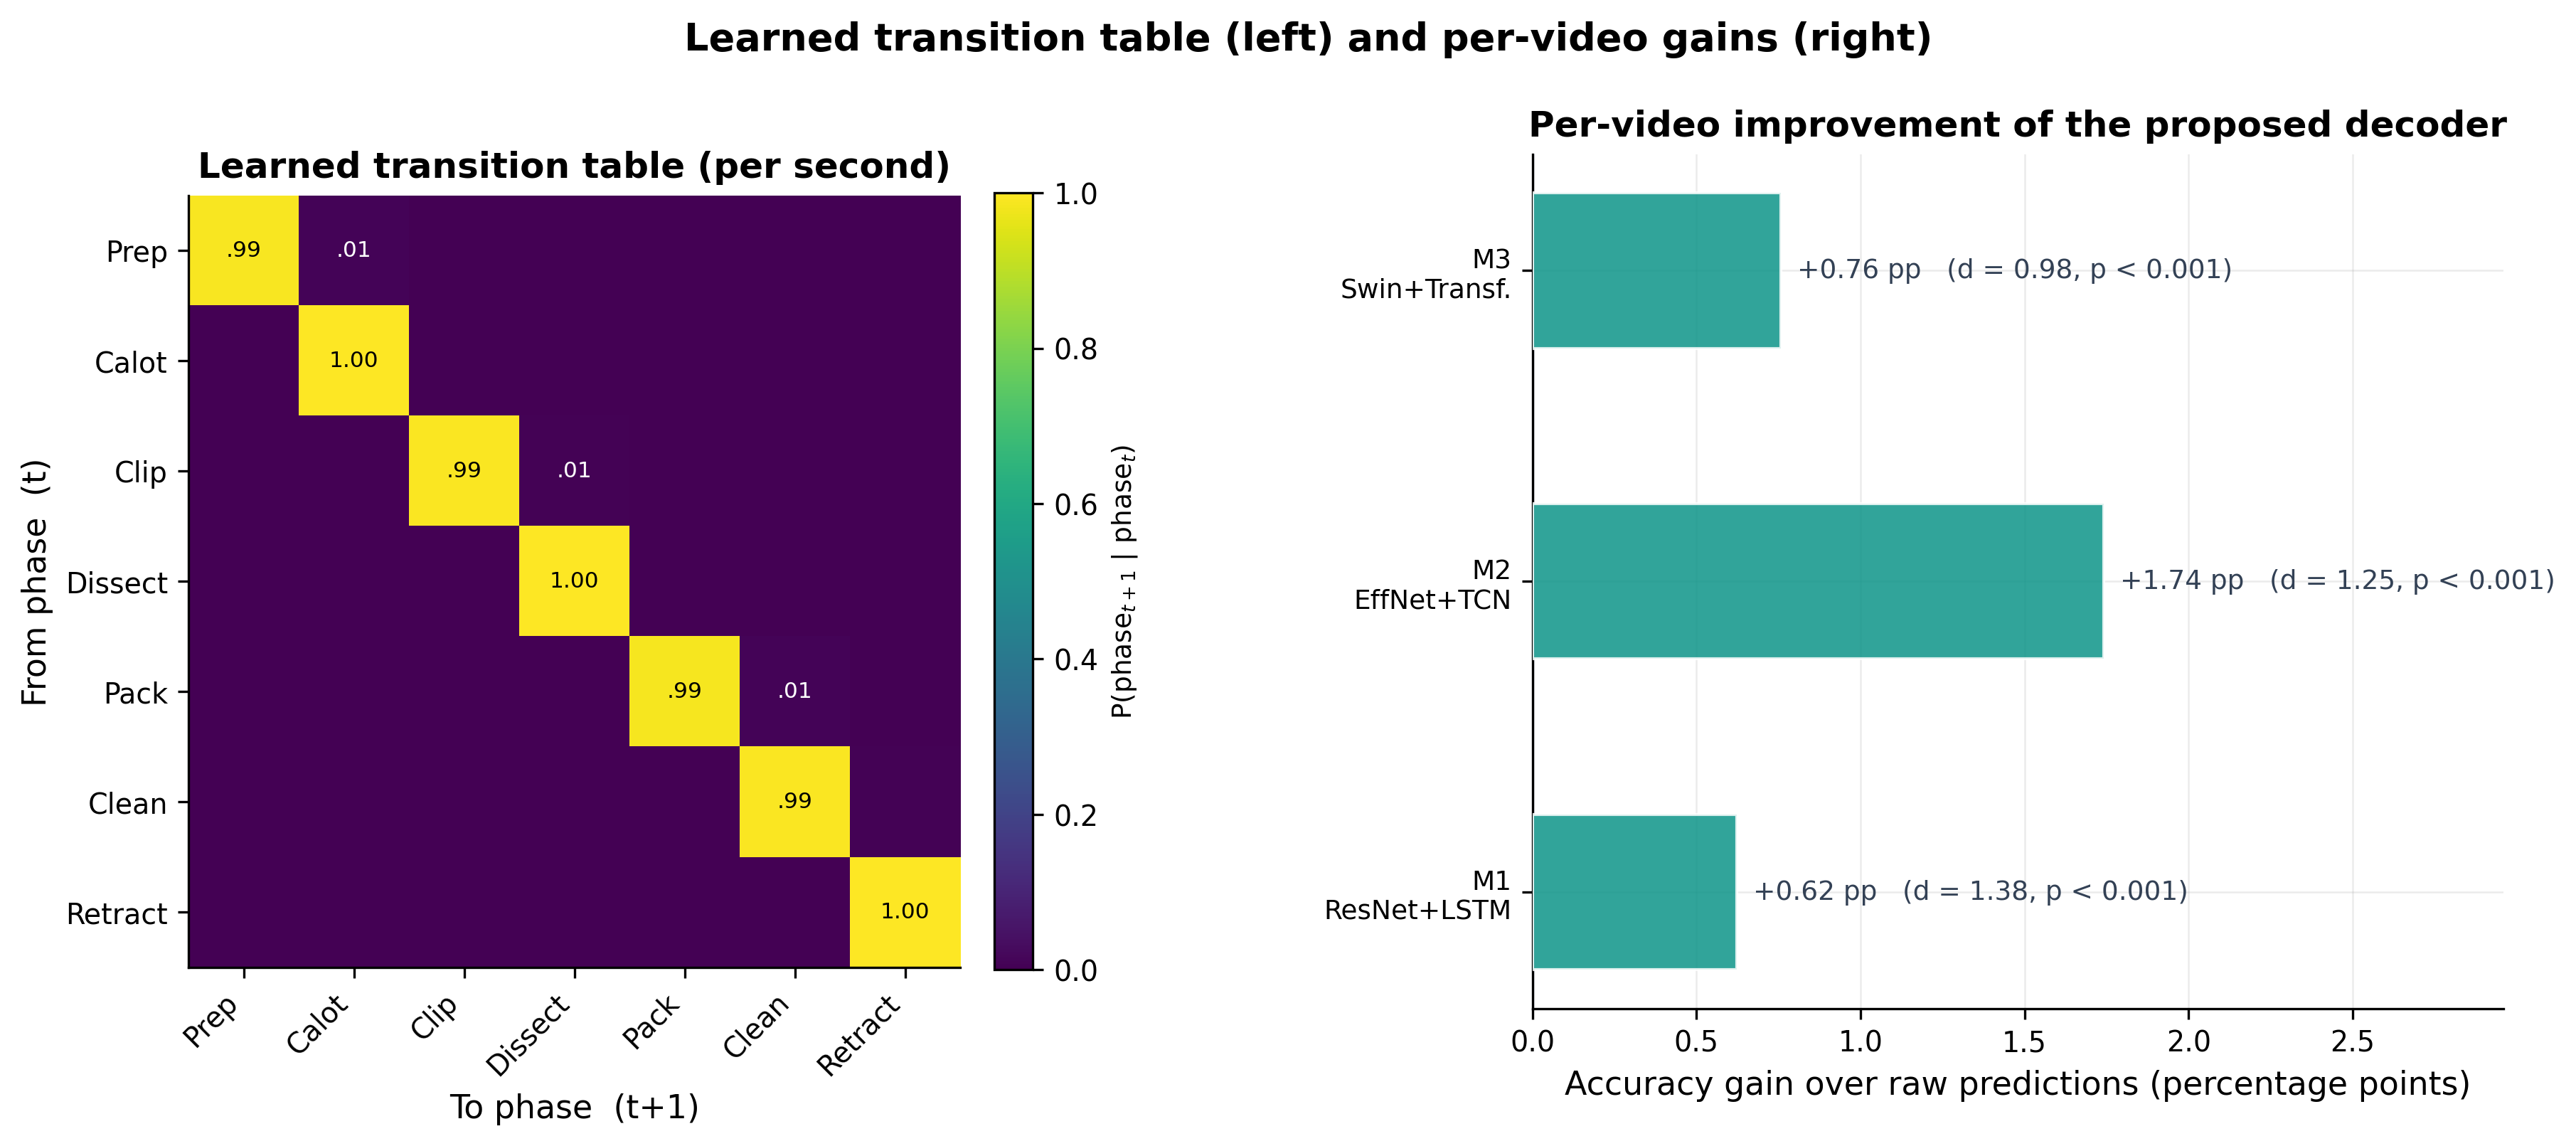
\includegraphics[width=\textwidth]{figures/transition_significance.png}
\caption{Trái: bảng chuyển pha mỗi giây học được, có đường chéo trội mạnh với phần trọng số còn lại nằm ở pha kế tiếp, khớp với trình tự pha cố định. Phải: mức tăng độ chính xác theo từng video của bộ giải mã đề xuất so với dự đoán thô, kèm hệ số Cohen $d$ và giá trị $p$ Wilcoxon.}
\label{fig:vn_transition_significance}
\end{figure}

\subsection{Ví dụ Minh họa}

Hình~\ref{fig:vn_timeline} cho thấy dòng thời gian pha dự đoán cho một video kiểm tra. Các dự đoán thô đổi qua đổi lại, nhất là ở đoạn đầu; bộ giải mã đề xuất loại bỏ phần lớn các lần đổi này và bám theo nhãn thật sát hơn nhiều.

\begin{figure}[H]
\centering
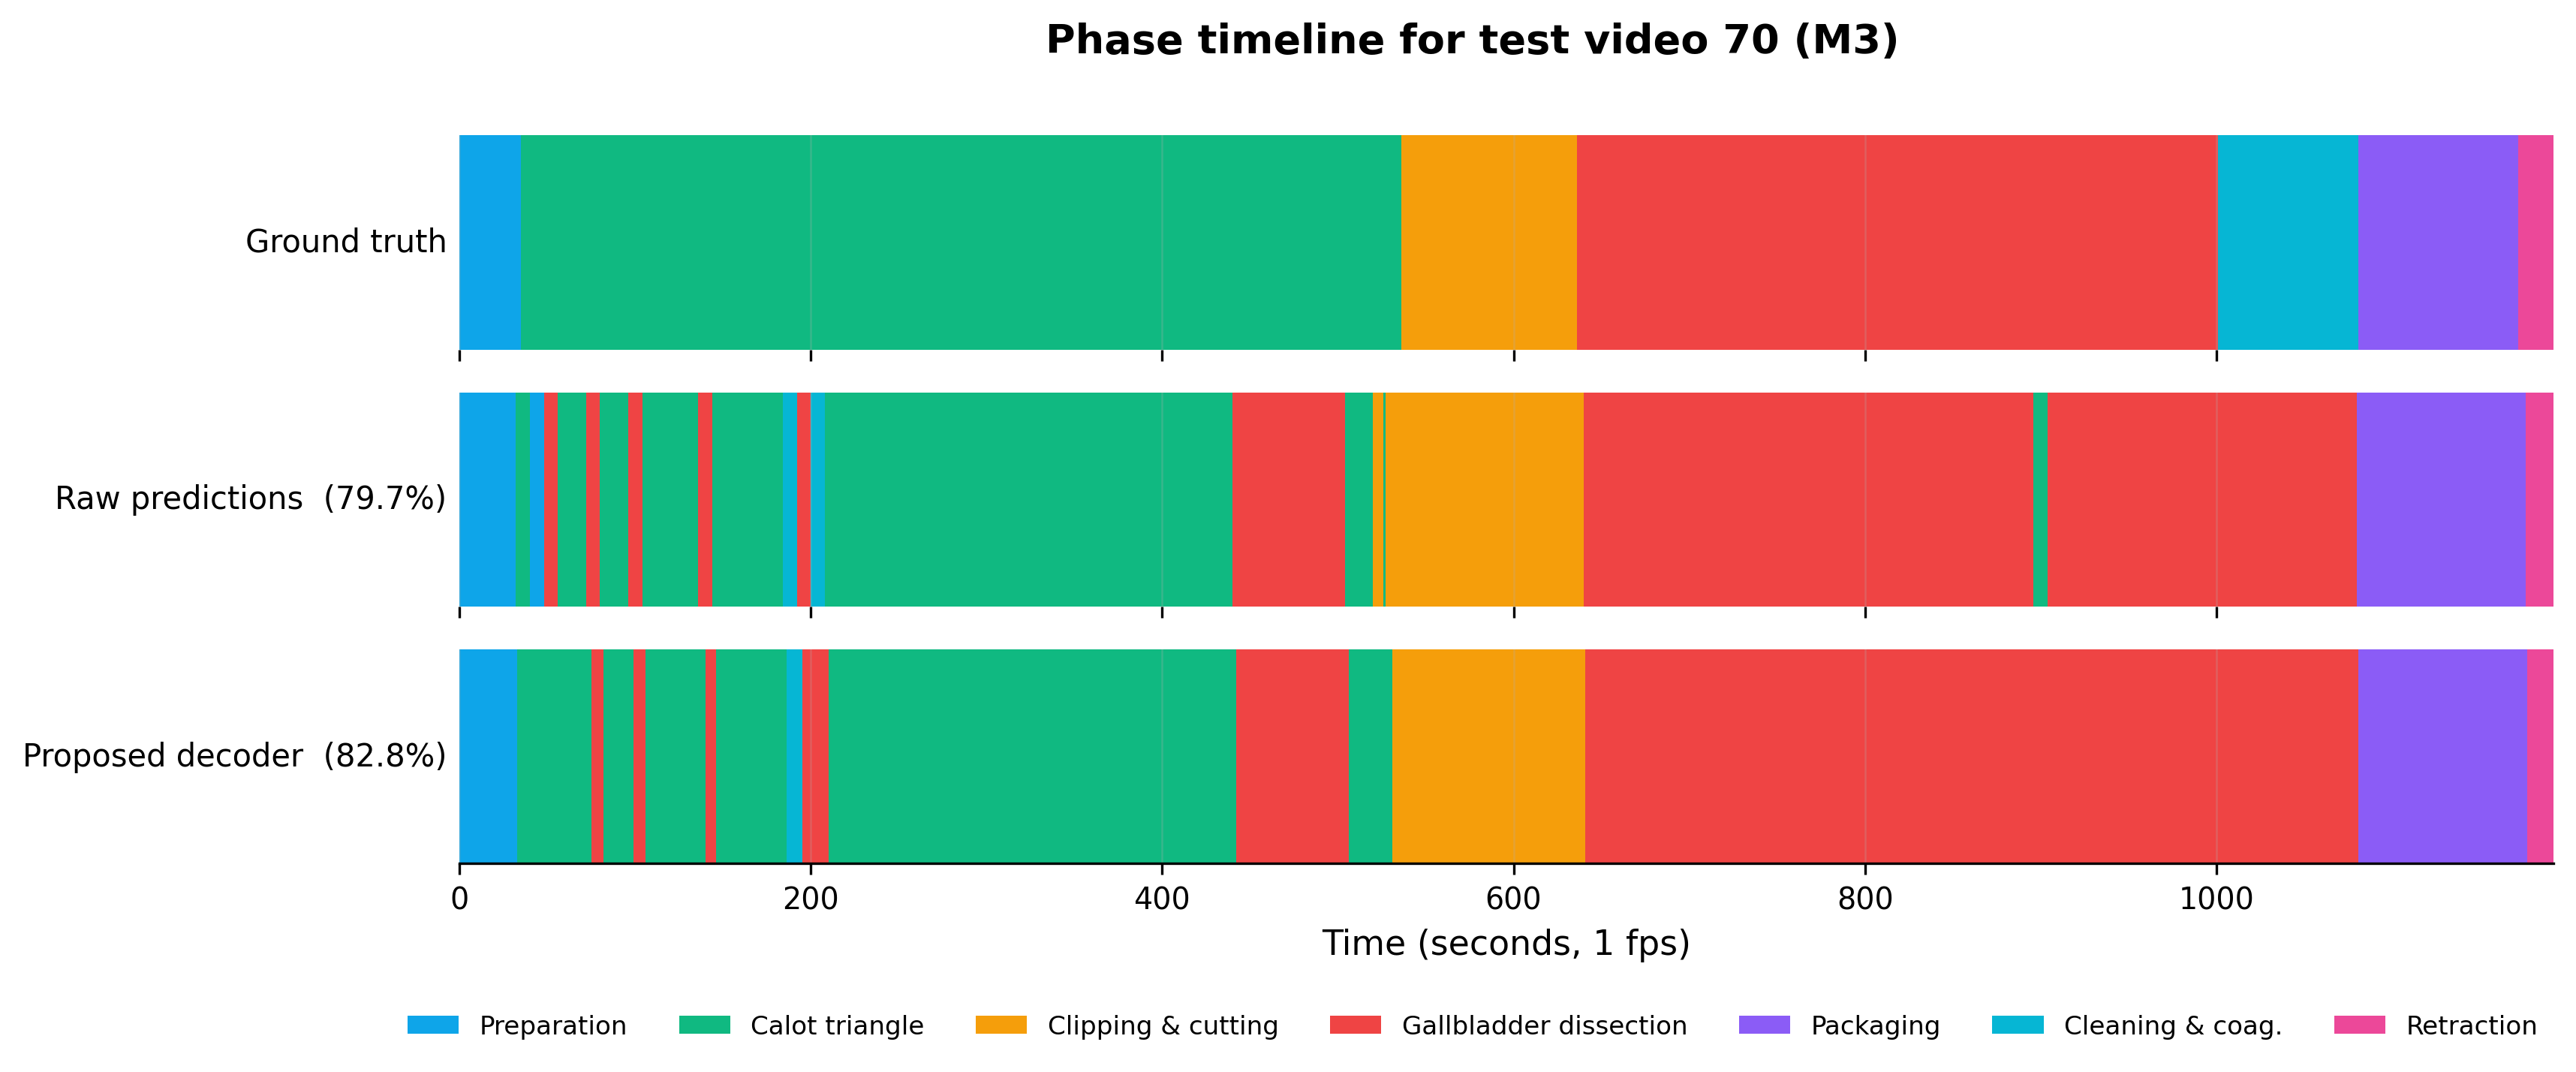
\includegraphics[width=\textwidth]{figures/timeline.png}
\caption{Dòng thời gian pha cho một video kiểm tra (M3). Các dự đoán thô (giữa) đổi nhãn thường xuyên; bộ giải mã đề xuất (dưới) mượt hơn hẳn và bám sát nhãn thật (trên).}
\label{fig:vn_timeline}
\end{figure}

\section{Lỗi Gần Điểm Chuyển pha so với Bên trong Pha}
\label{sec:vn_boundary}

Trên Cholec80, sự bất đồng về nhãn tập trung ở các điểm chuyển pha, nơi ngay cả người gán nhãn cũng khác nhau về thời điểm chính xác của chuyển tiếp. Để thấy mỗi bộ giải mã giúp ích ở đâu, các khung hình kiểm tra được chia thành nhóm \textbf{gần một điểm chuyển pha} (trong khoảng $\pm5$~giây quanh một chuyển tiếp thật) và nhóm \textbf{bên trong một pha} (mọi chỗ còn lại). Bảng~\ref{tab:vn_boundary} báo cáo cách chia này cho M3, và Hình~\ref{fig:vn_boundary} minh họa nó.

\begin{table}[H]
\centering
\caption{Độ chính xác gần điểm chuyển pha so với bên trong pha, cho M3. Bộ giải mã ngoại tuyến $\dagger$ dùng các khung hình tương lai. Giá trị \emph{thời gian thực} tốt nhất in \textbf{đậm}.}
\label{tab:vn_boundary}
\begin{tabular}{lcc}
\toprule
\textbf{Bộ giải mã} & \textbf{Gần chuyển pha} & \textbf{Bên trong pha} \\
\midrule
Dự đoán thô              & 60,7\% & 86,1\% \\
Lọc trung vị-15          & 61,1\% & 86,3\% \\
\textbf{Bộ giải mã đề xuất} & \textbf{63,2\%} & 86,8\% \\
\midrule
Ngoại tuyến (toàn video) $\dagger$ & 62,8\% & 91,0\% \\
\bottomrule
\end{tabular}
\end{table}

\begin{figure}[H]
\centering
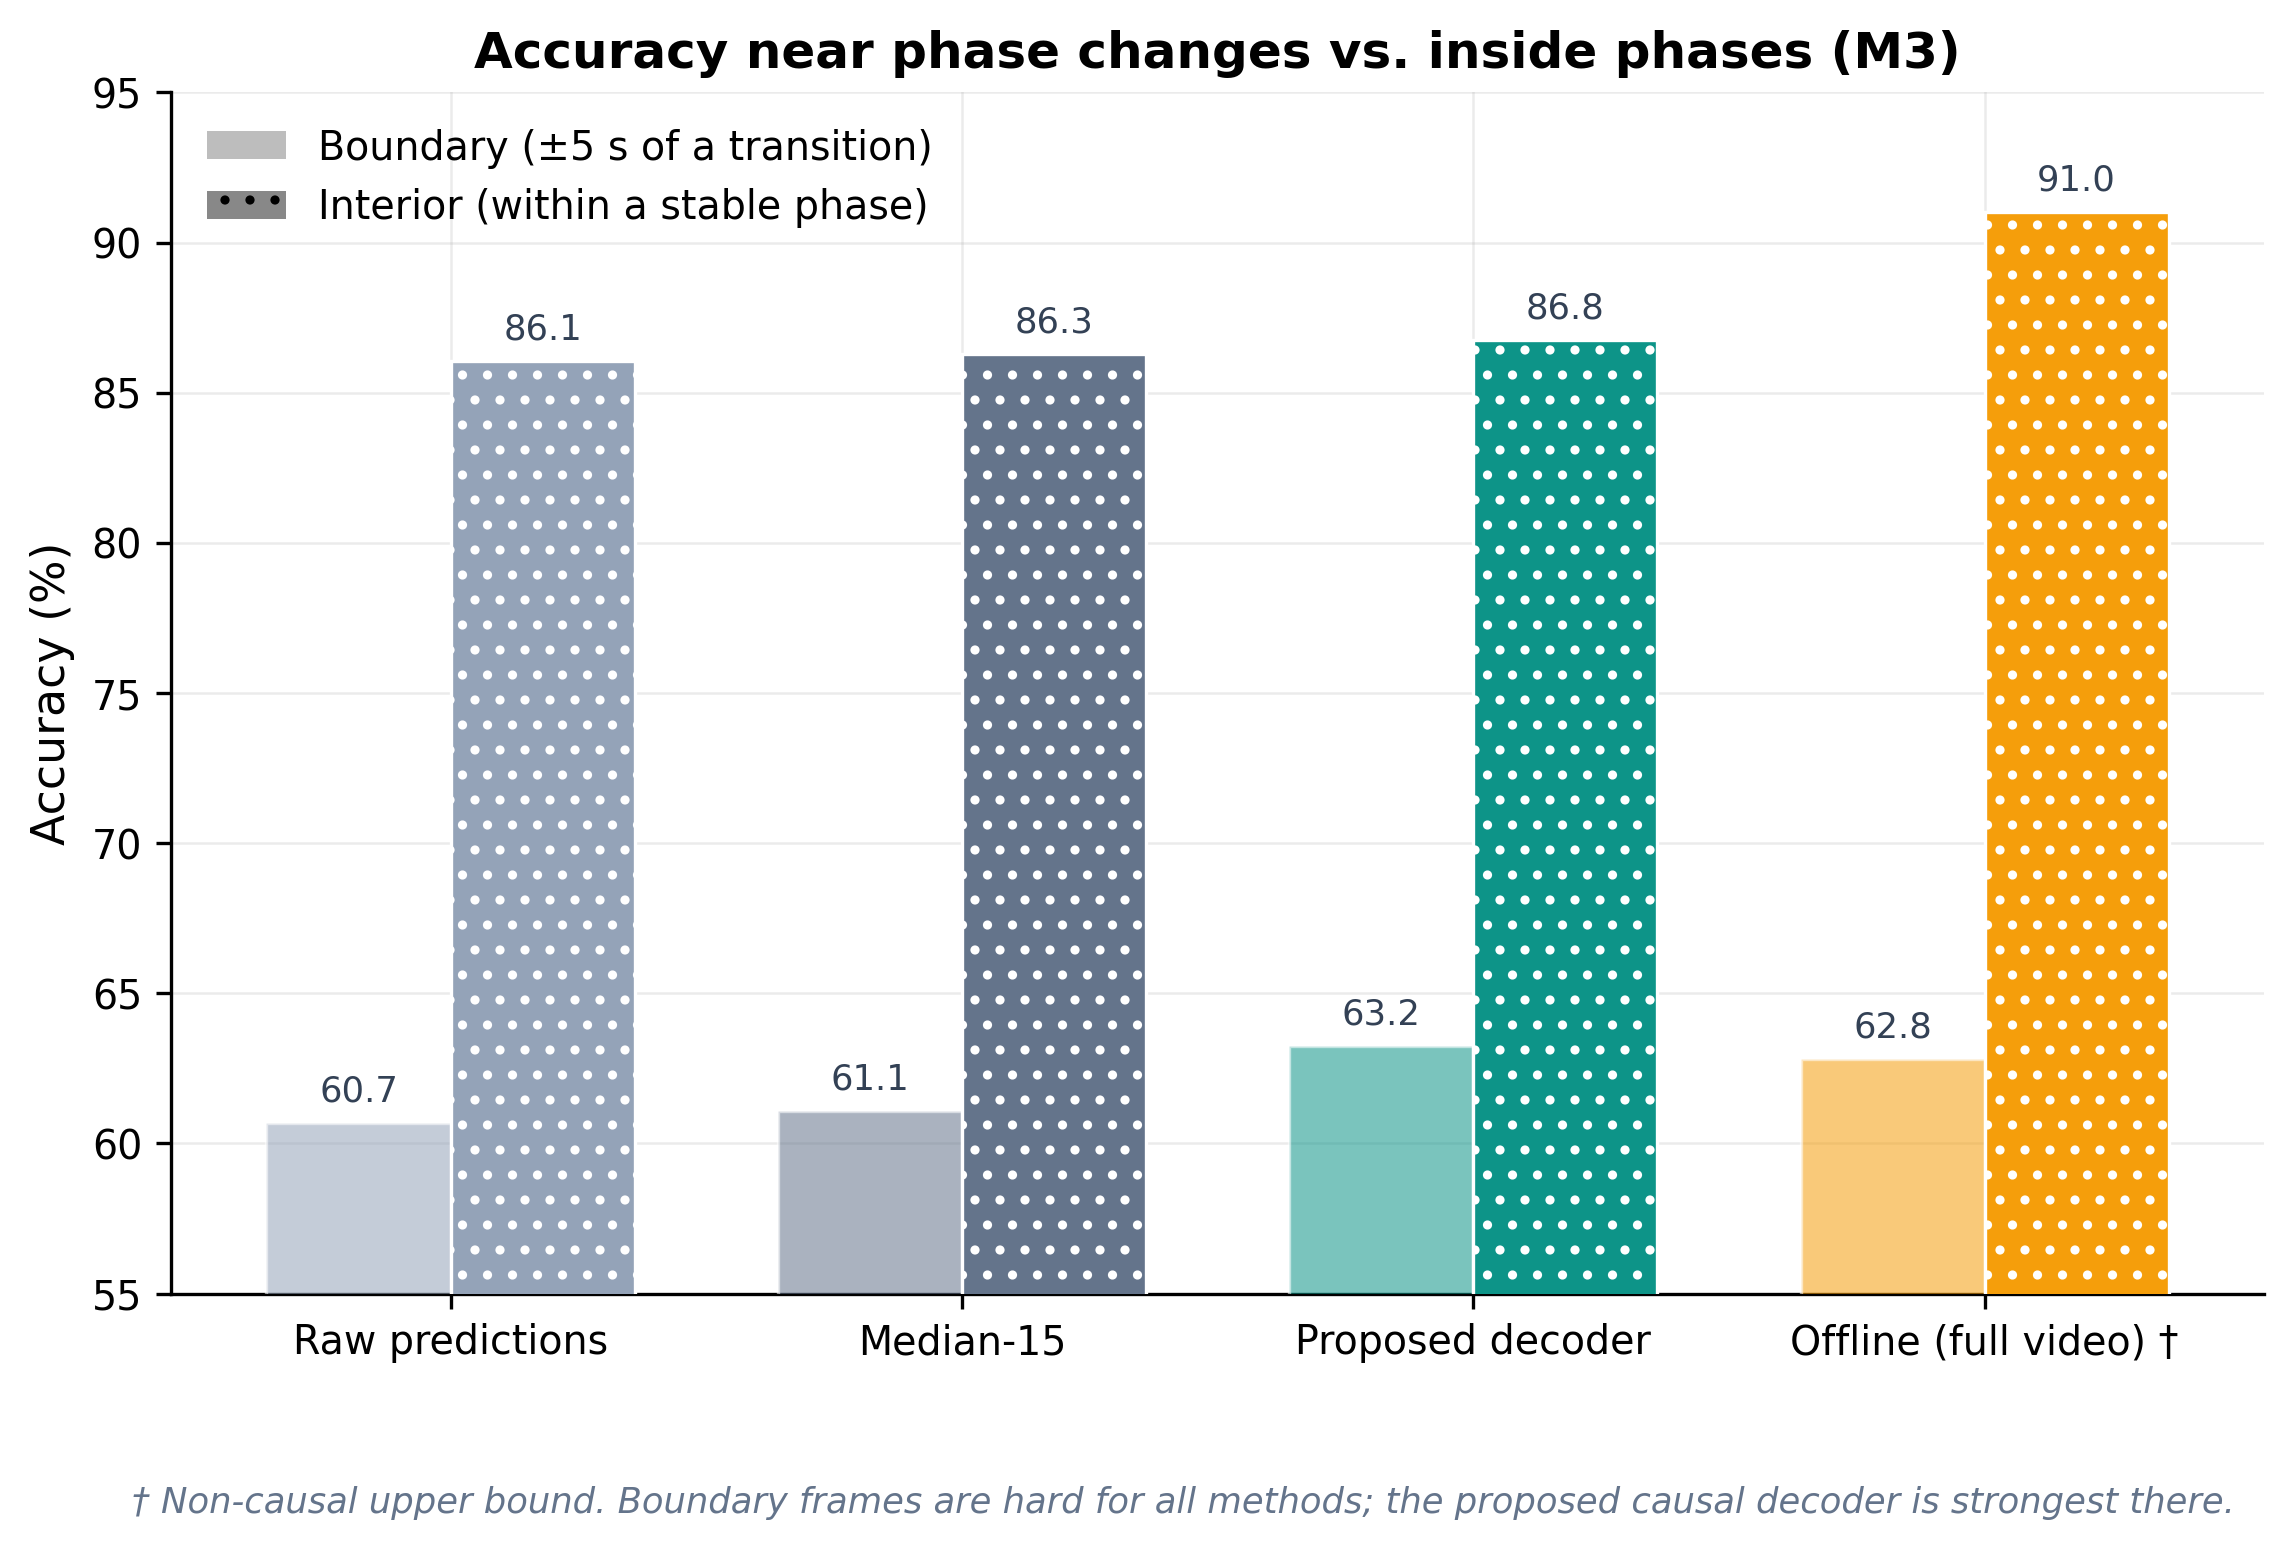
\includegraphics[width=\figwidth]{figures/boundary.png}
\caption{Độ chính xác gần điểm chuyển pha so với bên trong pha, cho M3. Các khung hình gần chuyển pha (cột đặc) khó với mọi phương pháp; bộ giải mã đề xuất tốt nhất ở đó, thậm chí hơi cao hơn cả cận trên ngoại tuyến. Bên trong pha (cột gạch chéo) là nơi ưu thế của bộ giải mã ngoại tuyến đến từ.}
\label{fig:vn_boundary}
\end{figure}

Hai điểm nổi bật. Thứ nhất, bộ giải mã đề xuất \textbf{tốt nhất ở gần điểm chuyển pha} (63,2\%), thậm chí trên cả cận trên ngoại tuyến (62,8\%): quy tắc cứng của bộ giải mã ngoại tuyến rằng pha không thể đi lùi đôi khi làm trễ một chuyển tiếp, trong khi bảng học được mềm dẻo hơn nên bám theo thời điểm chuyển nhãn linh hoạt hơn. Thứ hai, toàn bộ khoảng cách 4,2 điểm giữa bộ giải mã ngoại tuyến và bộ giải mã thời gian thực tốt nhất nằm \emph{bên trong} các pha ($86{,}8 \to 91{,}0$), không phải ở các điểm chuyển. Ưu thế của bộ giải mã ngoại tuyến là sửa các lỗi thoáng qua bên trong các pha dài ổn định bằng cách nhìn các khung hình tương lai --- điều mà một bộ giải mã thời gian thực không thể làm. Theo hiểu biết của chúng tôi, cách chia này chưa từng được đo trên Cholec80, và nó chỉ ra một bước tiếp theo rõ ràng: cho phép bộ giải mã nhìn trước vài giây sẽ thu hẹp phần lớn khoảng cách mà vẫn dùng được gần như thời gian thực.

% ======================= CHƯƠNG 5: KẾT LUẬN ==========================
\chapter{Kết luận và Hướng Phát triển}

\section{Tóm tắt Đóng góp}

Khóa luận này nghiên cứu nhận dạng pha phẫu thuật trên Cholec80 trên một GPU laptop duy nhất, xoay quanh hai phần gắn kết với nhau.

Phần thứ nhất là một \textbf{so sánh công bằng giữa ba kiến trúc}. ResNet-50~+~BiLSTM, EfficientNet-B3~+~TCN, và Swin-Tiny~+~Transformer được huấn luyện bằng một pipeline giống hệt nhau (lịch trình ba giai đoạn, tái cân bằng lớp, nhiệm vụ dụng cụ phụ, làm mượt nhãn, và huấn luyện độ chính xác hỗn hợp) trên một GPU 4~GB duy nhất. Giữ cố định công thức huấn luyện giúp tách riêng ảnh hưởng của kiến trúc: Swin-Transformer đạt Macro-F1 đã làm mượt là 0,815, cao hơn ResNet-LSTM 3,4 điểm và cao hơn EfficientNet-TCN 6,7 điểm. Bốn nghiên cứu loại bỏ sau đó cho thấy nhiệm vụ dụng cụ đáng giá khoảng $+1{,}6\%$ Macro-F1 và tái cân bằng lớp khoảng $+2{,}0\%$, còn việc kết hợp ba mô hình thêm 1,0 điểm nữa.

Phần thứ hai nhắm vào \textbf{bước giải mã và hiệu chuẩn} mà phần lớn công trình Cholec80 bỏ qua. Một bộ giải mã thời gian thực, kết hợp các dự đoán đã hiệu chuẩn nhiệt độ với một bảng chuyển pha học được, đã được thêm vào. Không cần huấn luyện lại các mô hình, nó nâng độ chính xác trên tập kiểm tra thêm $+0{,}6$ đến $+1{,}7$ điểm trên cả ba mô hình --- một mức tăng nhỏ nhưng, theo kiểm định ghép cặp, là rõ ràng và nhất quán --- với chi phí 0,013~ms mỗi khung hình. Việc tách lỗi cho thấy bộ giải mã mạnh nhất đúng ở nơi các mô hình yếu nhất (tại các điểm chuyển pha), và rằng phần khoảng cách còn lại so với cận trên ngoại tuyến nằm hoàn toàn bên trong các pha.

\section{Các Phát hiện Chính}

Ba phát hiện vượt ra ngoài tập dữ liệu và các mô hình cụ thể được nghiên cứu.

\textbf{Công thức huấn luyện quan trọng ngang với kiến trúc.} Đánh trọng số lớp và nhiệm vụ dụng cụ cộng lại đáng giá gần bốn điểm Macro-F1 --- gần bằng khoảng cách giữa kiến trúc tốt nhất và kém nhất. Trên một tập dữ liệu phẫu thuật mất cân bằng, cách huấn luyện mô hình quan trọng ngang với việc dùng mạng nền nào. Điều này dễ bị bỏ sót khi một so sánh thay đổi cả kiến trúc lẫn công thức cùng lúc, đó chính là điều mà pipeline cố định ở đây muốn tránh.

\textbf{Hiệu chuẩn là thứ làm cho bảng chuyển pha trở nên hữu ích.} Co giãn nhiệt độ thường được biện minh chỉ bằng độ tin cậy, nhưng ở đây nó có một vai trò thứ hai: bộ giải mã cộng các điểm số đã hiệu chuẩn với trọng số chuyển pha lại với nhau, nên nếu các điểm số quá nhọn thì bảng bị bỏ qua. Hiệu chuẩn các điểm số là thứ cho phép trình tự pha học được phát huy tác dụng, đó là lý do bộ giải mã có hiệu chuẩn luôn thắng bộ không hiệu chuẩn.

\textbf{Lợi ích của việc nhìn trước nằm bên trong các pha.} Ưu thế của bộ giải mã ngoại tuyến so với bộ giải mã thời gian thực tốt nhất gần như hoàn toàn là việc sửa các lỗi thoáng qua bên trong các pha dài, ổn định bằng các khung hình tương lai --- chứ không phải đặt các điểm chuyển pha chính xác hơn. Vậy nên một hệ thống thời gian thực hy sinh khả năng sửa các lỗi nhỏ bên trong pha, chứ không phải độ chính xác ở ranh giới. Do đó cho phép bộ giải mã nhìn trước vài giây là bước tiếp theo tự nhiên.

\section{Hạn chế}

Một số ràng buộc giới hạn các kết luận của nghiên cứu này:

\begin{itemize}
    \item \textbf{Phần cứng hạn chế.} GPU 4~GB buộc phải dùng kích thước lô và độ dài chuỗi nhỏ. Kết quả trên phần cứng lớn hơn có thể cao hơn một đến ba điểm, và riêng EfficientNet-TCN bị cắt ngắn giai đoạn tinh chỉnh thứ ba, nên các con số của nó là cận dưới chứ không phải một ước lượng công bằng.
    \item \textbf{Một tập dữ liệu.} Mọi kết quả đều từ Cholec80. Các quy trình có trình tự pha kém chặt chẽ hơn có thể cần một bảng chuyển pha lỏng hơn, và việc chuyển sang các ca phẫu thuật khác chưa được kiểm chứng.
    \item \textbf{Nhiễu nhãn ở điểm chuyển pha.} Thời điểm chính xác của mỗi chuyển pha trong Cholec80 không chính xác tuyệt đối, điều này đặt một trần lên độ chính xác đạt được ở gần điểm chuyển pha; trần này không được đo ở đây.
    \item \textbf{Lấy mẫu thưa trong bản demo trực tiếp.} Bản demo tương tác bỏ bớt khung hình để chạy nhanh, nên các pha kết thúc ngắn có thể bị bỏ sót ở tốc độ lấy mẫu thấp. Tuy nhiên, các con số benchmark được báo cáo dùng đầy đủ giao thức 1~fps và không bị ảnh hưởng.
\end{itemize}

\section{Hướng Phát triển}

Các hướng mở rộng trực tiếp nhất nhắm vào các hạn chế này:

\begin{itemize}
    \item \textbf{Nhìn trước trong độ trễ giới hạn.} Một bộ giải mã được phép nhìn trước vài giây sẽ thu hẹp phần lớn khoảng cách bên trong pha so với cận trên ngoại tuyến trong khi vẫn giữ độ trễ nhỏ, giải quyết đúng nút thắt tìm thấy ở Mục~\ref{sec:vn_boundary}.
    \item \textbf{Huấn luyện lại trên phần cứng lớn hơn.} Chạy lại đúng ba kiến trúc với lô lớn hơn và chuỗi dài hơn sẽ làm rõ bao nhiêu phần khoảng cách so với kết quả tốt nhất đã công bố là do phần cứng chứ không phải kiến trúc.
    \item \textbf{Ước lượng độ bất định.} Thêm dropout Monte-Carlo hoặc độ bất định dựa trên ensemble, bên trên việc hiệu chuẩn đã làm, sẽ cho mỗi dự đoán một giá trị độ tin cậy mà bác sĩ có thể dùng.
    \item \textbf{Các quy trình phẫu thuật khác.} Huấn luyện lại trên các ca phẫu thuật khác có nhãn quy trình sẽ kiểm tra xem pipeline và bộ giải mã dùng bảng học được có hoạt động ngoài ca cắt túi mật hay không.
\end{itemize}

Tóm lại, khóa luận này cho thấy có thể nhận dạng pha phẫu thuật tốt trên một GPU laptop thông thường khi huấn luyện, giải mã và hậu xử lý được thiết kế cùng nhau --- và rằng các bước giải mã và hiệu chuẩn, vốn thường bị xem là phụ, lại mang đến một cải thiện thực sự, đo lường được, và theo thời gian thực.


\end{document}
